\documentclass[
%a4paper,12pt
encoding=utf8
]{./twoeskd}

% Packages required by doxygen
\usepackage{fixltx2e}
\usepackage{calc}
\usepackage{doxygen}
\usepackage[export]{adjustbox} % also loads graphicx
\usepackage{graphicx}
\usepackage[utf8]{inputenc}
\usepackage{makeidx}
\usepackage{multicol}
\usepackage{multirow}
\PassOptionsToPackage{warn}{textcomp}
\usepackage{textcomp}
\usepackage[nointegrals]{wasysym}
\usepackage{hyperref}

% NLS support packages
\usepackage[T2A]{fontenc}
\usepackage[russian]{babel}

% Font selection
\usepackage{courier}
\usepackage{amssymb}
\usepackage{sectsty}
\renewcommand{\familydefault}{\sfdefault}
\newcommand{\+}{\discretionary{\mbox{\scriptsize$\hookleftarrow$}}{}{}}

% Page & text layout
\usepackage{geometry}
\tolerance=750
\hfuzz=15pt
\hbadness=750
\setlength{\emergencystretch}{15pt}
\setlength{\parindent}{0cm}
\setlength{\parskip}{0.2cm}
\makeatletter
\makeatother

% Headers & footers
% \usepackage{fancyhdr}
% \renewcommand{\sectionmark}[1]{%
%   \markright{\thesection\ #1}%
% }

% Indices & bibliography
\usepackage{natbib}
\usepackage[titles]{tocloft}
\setcounter{tocdepth}{3}
\setcounter{secnumdepth}{5}
\makeindex

% Custom commands
\newcommand{\clearemptydoublepage}{%
  \newpage{\pagestyle{empty}\cleardoublepage}%
}
\renewcommand{\DoxyLabelFont}{%
  \fontseries{bc}\selectfont%
}

% Custom packages
\usepackage{pdfpages}


\setlength{\parindent}{0cm}
\setlength{\parskip}{0.2cm}

\usepackage{listings}

% debug to see the frame borders
% from https://en.wikibooks.org/wiki/LaTeX/Page_Layout
% \usepackage{showframe}

% change style of titles in \section{}
\usepackage{titlesec}
\titleformat{\section}[hang]{\huge\bfseries\center}{\thetitle.}{1em}{}
\titleformat{\subsection}[hang]{\Large\raggedright}{\thetitle.}{1em}{\underline}
\titleformat{\subsubsection}[hang]{\large\raggedright}{\thetitle.}{1pt}{}

% Packages for text layout in normal mode
% \usepackage[parfill]{parskip} % автоматом делает пустые линии между параграфами, там где они есть в тексте
% \usepackage{indentfirst} % indent even in first paragraph
\usepackage{setspace}	 % controls space between lines
\setstretch{1} % space between lines
\setlength\parindent{0.9cm} % size of indent for every paragraph
\usepackage{csquotes}% превратить " " в красивые двойные кавычки
\MakeOuterQuote{"}


% this makes items spacing single-spaced in enumerations.
\newenvironment{my_enumerate}{
\begin{enumerate}
  \setlength{\itemsep}{1pt}
  \setlength{\parskip}{0pt}
  \setlength{\parsep}{0pt}}{\end{enumerate}
}

\newenvironment{my_itemize}{
\begin{itemize}
  \setlength{\itemsep}{1pt}
  \setlength{\parskip}{0pt}
  \setlength{\parsep}{0pt}}{\end{itemize}
}


% Custom commands
% configure eskd
\titleTop{
\textbf{\large ПРАВИТЕЛЬСТВО РОССИЙСКОЙ ФЕДЕРАЦИИ \\
ФЕДЕРАЛЬНОЕ ГОСУДАРСТВЕННОЕ АВТОНОМНОЕ \\
ОБРАЗОВАТЕЛЬНОЕ УЧРЕЖДЕНИЕ ВЫСШЕГО ОБРАЗОВАНИЯ \\
НАЦИОНАЛЬНЫЙ ИССЛЕДОВАТЕЛЬСКИЙ УНИВЕРСИТЕТ \\
«ВЫСШАЯ ШКОЛА ЭКОНОМИКИ» } \\
\vspace*{0.3cm}
\textnormal{\normalsize Факультет компьютерных наук \\
Департамент программной инженерии \\
}
}
\titleDesignedBy{\parbox[t]{7cm} {
Студент группы БПИ 151 \\
4 курса бакалавриата \\
образовательной программы \\
«Программная инженерия» \\
}}{А. M. Абрамов}
\titleAgreedBy{%
\parbox[t]{7cm} {
доцент департамента \\
программной инженерии \\
канд. техн. наук. \\
}}{С. Л. Макаров}
\titleApprovedBy{
\parbox[t]{10cm} {
Академический руководитель \\
образовательной программы \\
«Программная инженерия» \\
профессор департамента \\
программной инженерии \\
канд. техн. наук \\
}}{В. В. Шилов}
\titleName{\textbf{\Large Выпускная квалификационная работа} \\
\vspace*{0.6cm}
\textnormal{\large на тему \underline{Программа для управления и взаимодействия с реле времени РВ-90}\\
\vspace*{0.3cm}
по направлению подготовки 09.03.04 «Программная инженерия» \\
}}
\workTypeId{RU.02.11 01-1}
\workShortFullTitle{\small А. M. Абрамов. Программа для управления и взаимодействия с реле времени РВ-90}

\titleSubname{Пояснительная записка}


%===== C O N T E N T S =====
\begin{document}

% Titlepage & ToC
\pagenumbering{roman}

\textbf{\Large Реферат} \\

Данная работа посвящена реализации программы для управления и взаимодействия с реле времени РВ-90. РВ-90 это устройство для автоматизации включения и выключения промышленных или домашних приборов в зависимости от времени.

Приведен сравнительный анализ других реле времени, которые используются для автоматизации в промышленности. Выявлены преимущества и недостатки характерные для подобных устройств.

Разработанная программа имеет клиент-серверную архитектуру и состоит из трех модулей: прошивка устройства, веб-интерфейс и Android приложение. Программа позволяет пользователю настроить РВ-90 для решения задач автоматизации. Прошивка устанавливается на само устройство и управляет периферией. Веб-интерфейс предоставляется пользователю через канал Wi-Fi и обеспечивает взаимодействие. Android приложение дублирует и расширяет возможности веб-интерфейса для владельцев Android.

В качестве основных технологий используемых для разработки прошивки выступают язык С, официальный SDK от компании Realtek для микроконтроллера RTL8711AM и GNU инструменты сборки программ для ARM процессоров. Для разработки веб-интерфейса использовались технологии CSS, HTML, Javascript, для сборки и оптимизации файлов использовался инструмент Gulp. Для разработки Android приложения использовались язык Java и среда разработки Android Studio.

Работа содержит \pageref{LastPage} страниц, 3 главы, 21 рисунок, 19 источников, 4 приложения.

\textbf{Ключевые слова:} автоматизация,  микроконтроллеры, Wi-Fi, реле времени.

\newpage

\textbf{\Large Annotation} \\

This work is focused on the implementation of the program for control and interaction with the time relay RV-90. RV-90 is a device for automation of industrial or home appliances as a function of time.

The comparative analysis of other time relays, which are used for automation in industry, is given. Advantages and disadvantages typical for such devices are revealed.

The developed program has a client-server architecture and consists of three modules: device firmware, web interface and an Android application. The program allows the user to configure the RV-90 to solve the task at hand. The firmware is meant to be installed on the device, it purpose is to control the peripherals. The web interface is provided to the user via a Wi-Fi channel and allows for user interaction. Android app duplicates and extends the capabilities of the web interface for the convenience of Android owners.

The cornersone technologies used for firmware development are the C programming language, official SDK from Realtek for the RTL8711AM microcontroller and the GNU ARM toolchain. The web interface is build using CSS, HTML, Javascript. Gulp was used to bundle and optimize the web interface files. The Android application was developed in Android Studio in the Java programming language. 

The work contains \pageref{LastPage} pages, 3 chapters, 21 drawings, 19 sources, 4 attachements.

\textbf{Keywords:} automation, microcontrollers, Wi-Fi, time relay.



\newpage
\pagenumbering{arabic}
\tableofcontents
% \pagenumbering{arabic}

% --- add my custom headers ---
\setcounter{secnumdepth}{0}

\newpage
\section{Терминология}
\subsection{Терминология}
\begin{description}


\item[Реле времени]

Прибор производственно-технического или бытового назначения в заданный момент времени выдающий определенный сигнал либо включающий/выключающий какое-либо оборудование через свое устройство коммутации электросети. 

\item[Часы реального времени]

Электронная схема, предназначенная для учёта хронометрических данных (текущее время, дата, день недели и др.).


\end{description}



\newpage
\section{Введение}
\subsection{Введение}

В данном разделе представлено введение в предметную область, формулировка цели работы, а также новизна и практическая значимость работы.

Автоматизация - это технология, с помощью которой процесс или процедура выполняется с минимальным вовлечением человека. Некоторые процессы могут быть полностью автоматизированы. Автоматизация может быть востребована в самых разнообразных сценариях от термостата контролирующего бойлер загородного дома, до промышленной системы управления с набором исполнительных сигналов на выходе которые требуют высокой точности синхронизации по времени. Сложность решений варьируется начиная от простых элементов управления типа вкл/выкл и заканчивая алгоритмами, обрабатывающими сотни входящих сигналов каждую секунду. Преимущества автоматизации включают в себя экономию труда, экономию затрат на электроэнергию, экономию материальных затрат и повышение качества и точности исполнения процессов. В данной работе  рассматриваются простые системы автоматизации, которые характеризуются наличием часов реального времени (RTC) в качестве входа и от одного до четырех реле включения/выключения в качестве выходов. Такие устройства называются реле времени и обычно они делятся на 4 категории в зависимости от длительности временного интервала, для которого они позволяют устанавливать события включения/выключения: ежедневно, еженедельно, ежемесячно, ежегодно.

Устройства, которые в настоящее время доступны в нижнем и среднем ценовых  сегментах рынка, либо предоставляют очень ограниченный функционал, либо сложны в эксплуатации. Маленький LCD экран встречаемый на многих моделях серьезно ограничивает возможность вывода полезной информации пользователю. Для настройки, навигации по меню, а также для ввода всех числовых значений многие устройства предоставляют лишь кнопки на передней панели, что делает процесс медленным и подверженным ошибкам. Наконец, те редкие устройства, которые позволяют удаленное управление через компьютер или телефон, страдают от проблем с безопасностью соединения.

Тем не менее реле времени используются во многих отраслях, по оценкам компании ООО «Реле и Автоматика» годовой спрос на реле времени составляет примерно 20-30 тысяч[13].

Целью данной работы является разработка и реализация программы для управления и взаимодействия с реле времени РВ-90 (Реле и автоматика, Москва, Россия). РВ-90 это современное устройство для решения проблемы автоматизации с зависимостью от времени, которое направлено на то чтобы быть надежным и удобным в эксплуатации не компенсируя эти свойства дорогой ценой или сильно ограниченным функционалом. РВ-90 использует Wi-Fi и веб-технологии, которые позволяют пользователю со смартфоном подключиться и управлять реле с помощью отзывчивого, удобного интерфейса. На данный момент существует только инженерный дизайн устройства. Без программы для управления и взаимодействия данное реле использовать невозможно.



\setcounter{secnumdepth}{3}

\newpage
\section{Глава 1. Анализ устройств автоматизации}
В данном разделе представлен обзор и анализ различных задач для автоматизации с зависимостью от времени, а также аналогов реле времени РВ-90. В конце раздела составлен краткий обзор достоинств и недостатков реле времени с выводами.


\subsection{Область применения}
Автоматизация с зависимостью от времени может быть востребована во многих  ситуациях. Далее исследуются возможные применения реле времени в разных областях.

\subsubsection{Городское хозяйство}
В любом крупном городе освещение улиц и фасадов контролируется с точностью до минуты в соответствии с ежегодным календарем, утвержденным администрацией города. Отдельные архитектурные и исторические объекты, а также памятники обычно имеют свои утвержденные годовые графики подсветки[2]. И график включения/выключения отличается от уличного и должен быть введен в действие отдельно. В целях экономии электроэнергии световая реклама, подсветки вывесок магазинов и кафе переключается в ночной режим вечером и возвращается в дневной режим утром. В школах и других  учебных заведениях используют звонки, чтобы сигнализировать о начале или конце урока и перемены.


\subsubsection{Сельское хозяйство}
В сельском хозяйстве посевы необходимо поливать по определенному расписанию. Этот график отличается в зависимости от сорта растений. Для газонов используется отдельный график полива[3]. В теплицах по суточному графику может осуществляется подсветка растений. На птицефабриках подсветка и кормление также осуществляется по часам.


\subsubsection{Производство}
Заводы должны ежедневно включать кондиционер и отопление в рабочее время суток и выключать их в ночное время, автоматизация этого процесса еще больше осложняется тем, что время включения/выключения для таких систем различно в выходные, праздничные и сокращенные дни[4]. 


\subsection{Существующие решения}
На текущий момент на низком и среднем ценовых сегментах рынка существуют несколько типов устройств для автоматизации изложенных выше задач. Их можно разделить на две категории: механические реле и электронные реле.

\subsubsection{Механические реле}
Механические реле времени имеют простое внутреннее устройство. Механический диск вращается с периодом 24 часа и с помощью мелких дип-переключателей на диске можно задать время включения и выключения. Эти реле предельно просты в эксплуатации, однако недостатком является то, что в таком формате можно реализовать только суточные реле с циклом который повторяется каждые 24 часа (невозможно задать программу на 2 дня, на неделю, на год). И, также, проблема в том, что число включений и выключений ограничено количеством дип-переключателей на диске, и, как правило, наименьший промежуток времени между включением и выключением другими словами точность срабатывания реле, составляет 15 минут. Механические реле не имеют никакого программного обеспечения.

Многие известные производители электротехники выпускают подобные устройства[5]. 
Западные производители: ABB[6], Siemens[7], Legrand, Orbis, Еuroautomatica, Elko
Китайские производители: Chint, IEK и д.р.

Реле времени 2РВМ (рис 1.) является типичным реле с анкерным механизмом. Оно предназначено для управления двумя независимыми электрическими цепями на замыкание или размыкание[8].

\begin{figure}[h!]
    \centering
    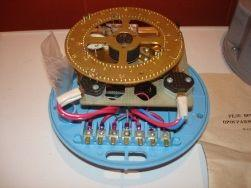
\includegraphics[width=0.5\textwidth]{mechanical_rele.png}
    \caption{Рисунок 1. Реле времени 2РВМ}
\end{figure}


\textbf{Преимущества}
\begin{my_enumerate}
\item Предельно просты в эксплуатации.
\item Надежны в работе.
\end{my_enumerate}

\textbf{Недостатки}
\begin{my_enumerate}
\item Программа только на 24 часа (нельзя задать программу на 2 дня, на год).
\item Число включений/выключений ограничено количеством дип-переключателей на диске.
\item Точность выбора времени включения/выключения - кратное 15 минут.
\end{my_enumerate}


\subsubsection{Электронные реле}
Наиболее распространенный тип реле времени, в основе которого используется микроконтроллер исполняющий загруженное в него программное обеспечение. Имеют различные входы и выходы для осуществления обратной связи, развитое программирование для задания необходимого алгоритма включений/выключений.  Поскольку в таких устройствах может использоваться кварцевая стабилизация частоты то они обеспечивают очень высокую точность[9]. В электронных реле можно задать программу работы на сутки, неделю и даже несколько лет. Можно выбрать время включения и выключения с высокой точностью до секунды, а количество событий включений и отключений которые можно запрограммировать в память реле измеряется сотнями. 

\subsubsection*{Реле на основе микроконтроллера}

Устройство которое использует LCD экран и кнопки управления для предоставления пользователю возможностей настройки.
Пример устройства РЭВ-302 (Новатэк-электро, Одесса, Украина) показан на рисунке 2.

\begin{figure}[h!]
    \centering
    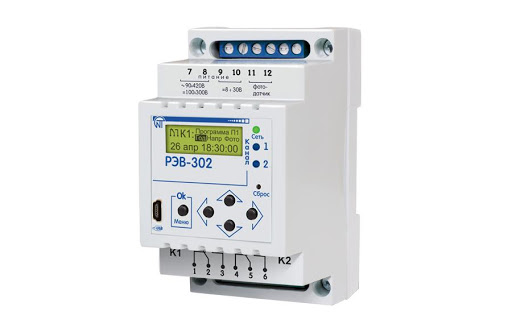
\includegraphics[width=0.5\textwidth]{rev302.png}
    \caption{Рисунок 2. Прибор РЭВ-302}
\end{figure}


РЭВ-302 можно настроить для включения и выключения периферийного прибора, например бойлера, в загородном доме в зависимости от точной даты и времени. Однако РЭВ-302 и аналоги излишне сложны в настройке.  Маленький LCD экран серьезно ограничивает возможность вывода полезной информации пользователю. Для настройки, навигации по меню, а также для ввода всех числовых значений имеются лишь несколько кнопок на передней панели, что делает процесс медленным и подверженным ошибкам. Устройство не предоставляет опции из коробки для удаленной работы. Получить обзор текущей конфигурации также очень сложно, что затрудняет работы по техническому обслуживанию и поддержке. Наконец, пользователь должен быть хорошо знаком с объемной инструкцией к изделию, для того чтобы успешно перемещаться по меню параметров и конфигурации. 

Реле времени РЭВ-302 выделяется тем что имеет micro-USB порт и поддерживает технологию USB-OTG. Таким образом данное реле можно настраивать с компьютера или с телефона/планшета[10]. Однако есть серьезные ограничения с поддержкой различных конфигураций операционных систем и платформ.

При настройки с ПК требуется наличие строго ОС Windows, а также наличие специальной программы для Windows от Новатэк-электро. При настройке с телефона/планшета требуется наличие строго ОС Android, а также наличие специального приложения для Android от Новатэк-электро. Любые другие конфигурации операционных систем и платформ не поддерживаются.

\textbf{Преимущества}
\begin{my_enumerate}
\item Можно задать программу работы на сутки, на неделю или на год.
\item Точность выбора времени включения/выключения - кратное секунде
\item Очень большое количество событий для включений и отключений.
\end{my_enumerate}

\textbf{Недостатки}
\begin{my_enumerate}
\item Маленький экран.
\item Объемная инструкция.
\item Очень неудобно программировать.
\item Затруднены работы по техническому обслуживанию и поддержке, если надо что-либо проверить/поменять в настройках.
\item Высокая цена
\end{my_enumerate}


\subsubsection*{Реле на основе микроконтроллера со встроенным модулем Wi-Fi}

Устройство которое использует сети Wi-Fi для предоставления пользователю возможности удаленной настройки и удобного интерфейса. 

Наиболее схожим с РВ-90 является линейка изделий Sonoff (Айтихэд Интеллектуальные Системы, Шэньчжэнь, Китай). Это очень бюджетные реле времени которые могут быть сопряжены со смартфоном посредством приложения eWeLink доступного на мобильных платформах. 

Однако у них есть и некоторые существенные недостатки. Во-первых, настройка реле происходит только через мобильное приложение eWeLink, из за чего данное реле невозможно настроить через ПК. Во-вторых, устройства Sonoff требуют подключения к интернету поскольку взаимодействие между пользователем и реле осуществляется через облачный сервер. Это может приводить к задержкам и сбоям в срабатывании реле.  Доступ к сети интернет делает их уязвимыми для атак.  Этот факт особенно важен учитывая что в устройствах Sonoff был обнаружен ряд серьезных уязвимостей, позволяющих используя механизм обновления по воздуху (OTA) обновить или полностью заменить заводскую прошивку реле без ведома или одобрения владельца. Также известно что устройства Sonoff не проверяли SSL-сертификаты на достоверность хотя они использовали HTTPS[11] соединение. Данного рода уязвимости позволяют проводить атаки направленные на перехват или манипуляцию команд обмениваемых между пользователем и устройством.

\textbf{Преимущества}
\begin{my_enumerate}
\item Можно контролировать удаленно
\item Точность выбора времени включения/выключения - кратное секунде
\item Достаточно большое количество событий для включений и отключений.
\item Невысокая цена
\end{my_enumerate}

\textbf{Недостатки}
\begin{my_enumerate}
\item Необходим доступ в интернет
\item Зависимость от облачных сервисов
\item Нет возможности настроить с ПК, только из приложения eWeLink
\item Проблемы с безопасной передачей данных через интернет
\end{my_enumerate}


\filbreak
\subsection{Определение характеристик желаемого решения}

Рассмотрев различные реле времени, можно составить краткий обзор достоинств и недостатков электронных реле времени, а также выделить важные характеристики которые будут важны при проектировании архитектуры системы.


При планировании архитектуры программы для управления и взаимодействия с реле времени РВ-90 следует учесть следующие требования:
\begin{my_itemize}
\item Безопасность и стабильность работы системы первостепенны.
\item Программа должна иметь максимально простой и интуитивный интерфейс. Т.к. механические реле все еще используются именно из-за их простоты в настройке.
\item Программа должна предоставлять возможность настройки с экрана ПК или мобильного телефона.  
\item Необходима поддержка различных конфигураций операционных систем и платформ. Нет смысла поддерживать только одну из многих платформ.
\item Программа не должна быть зависимым от облачного сервера.
\item Для снижения цены изделия отлично подойдет микроконтроллер со встроенной периферией Wi-Fi.
\item Программа должна поддерживать большое количество событий включений/выключений с точностью до секунды.
\end{my_itemize}


\subsection{Выводы по главе}
Для более глубокого понимания специфики индустрии были рассмотрены процессы которые могут быть автоматизированы с помощью реле времени. Помимо этого были рассмотрены наиболее часто применяемые изделия вместе с их сильными и слабыми сторонами. В результате пополнен состав требований к программе.








\newpage
\section{Глава 2. Описание выбранных методов}
Описание выбранных методов, моделей, алгоритмов решения задач.
Во-первых описывается общая трехкомпонентная архитектура программы.
Во-вторых с аппаратной точки зрения описываются платформы на которых будут исполнятся компоненты программы.
В-третьих описывается архитектура каждого компонента и их модулей.
В-четвертых описывается модель взаимодействия между модулями внутри каждого компонента.
В-пятых описывается модель взаимодействия между тремя компонентами программы.

\subsection{ Архитектура программы }
Программа имеет трехкомпонентную архитектуру. Первым компонентом является прошивка, устанавливаемая на РВ-90. Второй компонент представляет собой одно-страничное веб-приложение, которое будет храниться во флеш-памяти вместе с прошивкой, передаваться на устройство пользователя при подключении и запускаться в браузере. Третий компонент - это Android-приложение, которое может быть установлено на устройстве пользователя через Google Play[12]. Каждый компонент создается с использованием своего стека технологий. Таким образом, программа состоит из трех отдельных компонентов, которые должны быть разработаны отдельно и должны будут взаимодействовать друг с другом. 

Одним из основных факторов успеха мобильного приложения является простота его  распространения.  В связи с этим была выбрана мобильная операционная система  Android – самая распространенная мобильная операционная система для смартфонов, имеющая долю рынка около 80\%.
 
 
 
Конструкция аппаратной базы для РВ-90 является фиксированной и должна учитываться при проектировании архитектуры программы

\textbf{Три платформы}
\begin{my_itemize}
\item РВ-90
\item Браузер
\item Android
\end{my_itemize}


\begin{figure}[h!]
    \centering
    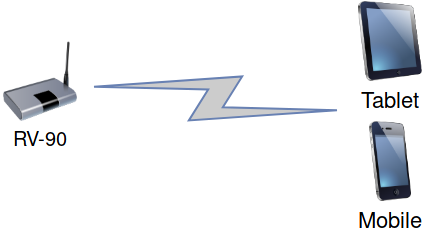
\includegraphics[width=0.9\textwidth]{three_platforms.png}
    \caption{Диаграмма взаимодействия между реле и клиентом.}
\end{figure}



%===========================================================================



\newpage
\subsection{ Платформа РВ-90 }
Аппаратная база представлена в виде устройства РВ-90. Нет смысла рассматривать абсолютно все физические характеристики устройства. Далее будут рассмотрены те из них, которые влияют на реализацию программы. В основе устройства находится модуль RAK473. К GPIO вводам которого подключены: 3 пина для программирования (SWDIO, SWCLK, RST), 2 пина для взаимодействия через UART (RX, TX), питание 5 вольт, земля, шина I2C. К шине I2C подключены часы реального времени DS1307 и I2C расширитель портов PCA9555. К GPIO выводам расширителя подключены 4 светодиода, 3 push-down кнопки, 2 реле RT424005.
Выбор компонентов влияет на архитектуру программы. В данной секции в больших деталях рассмотрены некоторые компоненты РВ-90 и их аналоги с целью понимания специфики каждого компонента. 

\subsubsection{ Кнопки на корпусе РВ-90 }
На корпусе имеются 3 кнопки, 2 из них для ручного переключения состояния каждого из двух реле, и одна для жесткой перезагрузки системы.
Кнопки не используют пин прерывания имеющийся у I2C расширителя портов RCA9555 для оповещения об изменении своего состояния. Программа должна периодически опрашивать текущее напряжение на кнопках, чтобы заметить нажатие. По умолчанию линии кнопок притянуты вверх, поэтому напряжение уровня земли соответствует нажатию. Программа должна применять фильтр к данным о состоянии кнопок, чтобы исключить ложные срабатывания, а также и двойные/тройные срабатывания из-за дребезжания контактов. 

\subsubsection{ I2C расширитель портов PCA9555} 
Выбор I2C расширителя портов PCA9555 обоснован его низкой ценой и расширением на 16 GPIO портов, которых более чем хватает для контроля аналоговой периферии. Выбор также обусловлен возможностью задать I2C адрес для расширителя на этапе производства устройства, чтобы избежать конфликта адресов на шине. В качестве аналога существует более дешевый PCA9554 предоставляющий расширение на 8 GPIO портов и имеющий жестко зафиксированный адрес на шине. 

\subsubsection{ Часы реального времени DS1374}
Выбор часов реального времени DS1374 имеет недостаток в виде высокой цены и много достоинств. 
Для взаимодействия с микроконтроллером данные часы используют протокол I2C, вместе с другой периферией их можно подключить к общей шине I2C, что очень важно в условиях ограниченного количества GPIO пинов  микроконтроллера.
Данные часы отсчитывают время в формате Unix-time. Формат Unix-time удобен для хранения, сравнения и передачи. Поскольку подразумевается что пользователь может создавать много событий включения/выключения требующих хранения времени, а память в системе ограничена, то важно иметь компактный формат для хранения времени. При взаимодействии с пользователем и при работе программы временные значения будут часто передаваться между различными программными модулями, важно что формат Unix-time очень прост в представлении и следовательно удобен для передачи. При принятии решений система должна уметь возможность сравнивать и считать разницу между двумя временными значениями, время в формате Unix-time можно удобно и быстро сравнивать между собой (простое сравнение 32-битных целых чисел). Недостатком формата Unix-time в том что он не может отразить дополнительные високосные секунды [\url{https://stackoverflow.com/a/50910322/1073672}], а также в том что он может отображать только даты в промежутке с 1901 по 2038 год. Также в январе 2038 года данный формат будет подвержен ошибке из-за переполнения 32-битного целого числа. Программа для управления РВ-90 работает лишь с текущим годом, плюс-минус 10 лет, поэтому в данной работе ошибка переполнения никак не обрабатывается. Что касается дополнительных високосных секунд, то с 1970 по 2007 их было 23 [\url{http://pubs.opengroup.org/onlinepubs/9699919799/xrat/V4_xbd_chap04.html#tag_21_04_15}], поэтому за период эксплуатации устройства, составляющий ориентировочно 2 года ожидается что их влияние будет несущественно. Тем не менее программа предоставляет пользователю возможность синхронизировать время в РВ-90 с другим устройством с целью устранения ошибки в отсчете времени на РВ-90. Часы DS1374 также имеют возможность генерировать программируемое прерывание.
Прерывания в определенный момент времени можно использовать для максимально точного контроля реле. Однако, в такой точности нет необходимости поскольку текущее время с точностью до секунды можно отсчитывать центральным процессором. Поэтому часы используются для борьбы с небольшой плавающей ошибкой, для этого программа синхронизируется с часами один раз в час. Также часы используются для бесперебойного отсчета времени когда устройство РВ-90 не подключено к электропитанию, для этого часы имеют отдельное питание от батарейки. Надо учитывать что часы используют 32-битное знаковое целое число для счетчика и подвержены ошибке переполнения счетчика в 2038 году. В данной работе эта ошибка не обрабатывается.  
В качестве аналога к часам DS1374 имеются часы DS1672, которые практически идентичны за исключением возможности генерации прерывания. 
Программа не имеет функционала для работы с часами использующими представление времени в формате BCD (Binary Coded Decimal). Часы в формате BCD удобны для вывода времени, кроме того они корректно отсчитывают текущую дату и время, принимая в расчет високосные года. В частности дополнительный день и секунды в високосный года, а также количество дней в каждом месяце в зависимости от текущего года. 
Пример часов работающих в формате BCD - DS1307, отличаются низкой ценой.


\subsubsection{ Wi-Fi модуль РАК473 }
Производства компании Rak-Wireless [\url{http://docs.rakwireless.com/en/WIFI/RAK473/Hardware%20Specification/RAK473%C2%A0UART%C2%A0WiFi%C2%A0Module%C2%A0Specification%20V1.5.pdf}]. 
Существует аналогичный модуль компании FN-link F11AMIM13\_B1. RAK473 включает в себя микроконтроллер RTL8711AM от Realtek, флеш-память GD25Q16C размером в 2MB от GigaDevice подключаемую к микроконтроллеру через SPI интерфейс, Wi-Fi антенну, регуляторы и предохранители для GPIO пинов чипа. Блок схема модуля представлена на рисунке.

\begin{figure}[h!]
    \centering
    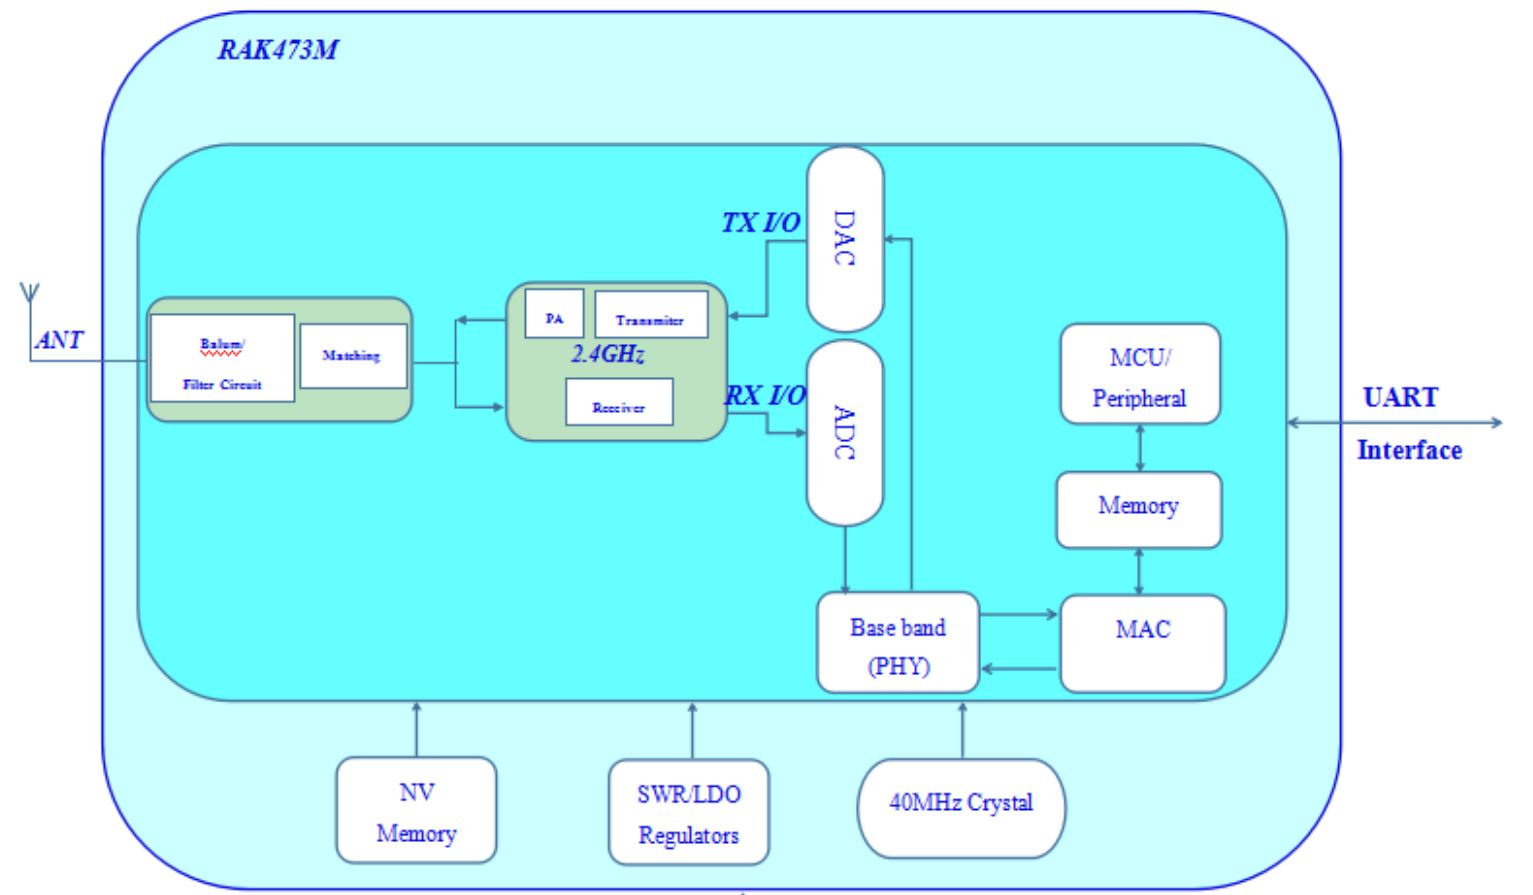
\includegraphics[width=0.9\textwidth]{rak473_block_diagram.png}
    \caption{Блок схема модуля на рисунке.}
\end{figure}

У модуля имеются 19 GPIO. 
Выводы GPIOB0 и GPIOB1 используются для UART.
Выводы GPIOB2, GPIOB3 используются для подключения шины I2C.
Выводы GPIOE4, GPIOE3 используются для программирования.
Схема GPIO выводов модуля представлена на рисунке.

\begin{figure}[h!]
    \centering
    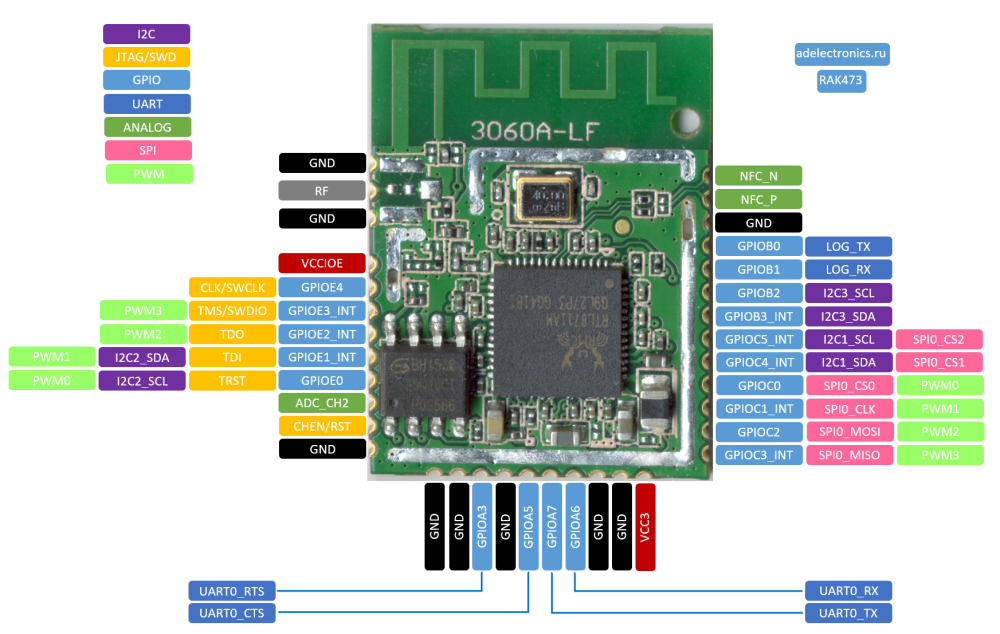
\includegraphics[width=0.9\textwidth]{rak473_pinout.png}
    \caption{Схема GPIO выводов модуля RAK473.}
\end{figure}

\subsubsection{ Микроконтроллер RTL8711AM}
В основе модуля RAK473 находится микроконтроллер производства компании Realtek[7]. Это одно-кристальный микропроцессор нацеленный для изделий Internet of Things. Он сочетает в себе ARM ядро на базе Cortex-M3, WLAN MAC и NFC в одном чипе. Тактовая частота процессора 166 MHz. 

Процессор имеет 1MB встроенной ROM памяти, 2.5 MB RAM памяти и SPI интерфейс для подключения Flash памяти.  В памяти ROM размещается заводской бутлоадер и некоторые функции для стандартной библиотеки. Данная память находится по адресам с 0х00000000 по 0х000FFFFF. Ей невозможно воспользоваться для разработки, т.к. ее невозможно перепрошить. Память RAM состоит из блока SRAM и блока SDRAM. SRAM (Static Random Access Memory) это статичная память, доступ к ячейкам данного типа памяти осуществляется быстрее чем к ячейкам памяти SDRAM (Synchronous Dynamic Random Access Memory), к тому же ее не надо периодически обновлять чтобы поддерживать правильные значения битов памяти. Однако она дороже т.к. требует большего количества транзисторов на один бит памяти. Поэтому в данном микроконтроллере память SRAM имеет всего лишь 448KB. SRAM расположена по адресам с 0х10000000 по 0х1006FFFF. Память SDRAM имеет 2 МB памяти. Доступ осуществляется по адресам с 0х30000000 по 0х301FFFFF.

При записке микроконтроллер начинает с исполнения заводской программы, то есть загрузчика (bootloader) находящегося в ROM памяти. Загрузчик инициализирует некоторые внутренние значения и переходит к считыванию данных из подключенной флеш-памяти. Ожидается что память подключена по протоколу SPI к определенным пинам микроконтроллера. 
Ниже представлено разбиение флеш-памяти с которым ожидает работать загрузчик. Изображение ниже не является картой RAM памяти. 

\begin{figure}[h!]
    \centering
    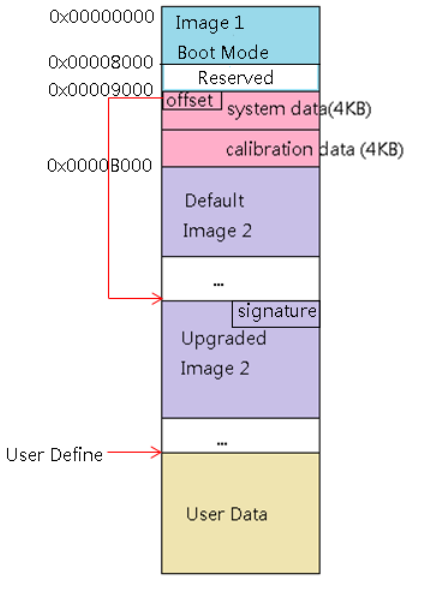
\includegraphics[width=0.4\textwidth]{rtl8711am_flash_layout.png}
    \caption{Разбиение флеш-памяти с которым ожидает работать загрузчик.}
\end{figure}

На схеме также показан "Upgraded Image 2", который используется для технологии обновления прошивки OTA (Over The Air). Данная программа не предусматривает возможности обновления прошивки по каналу Wi-Fi, поэтому область выделенная для "Upgraded Image 2" может быть использована для любых других нужд разработчика. В частности для хранения пользовательской информации.


Загрузчик поддерживает работу с форматом Binary Image File (.bin). Для того чтобы получить прошивку (файл типа .bin) которая будет правильно обработана загрузчиком следует использовать официальный SDK (Software Development Kit) от компании Realtek. Загрузчик читает данные из флеш-памяти и в соответствии с директивами формата ELF копирует данные в разные области RAM памяти. После этого загрузчик очищает свой стек и передает управление пользовательскому коду. Таким образом RTL8711AM не использует технологию XiP (Execute in Place), хотя она и является довольно распространенным решением.

\subsubsection{ Ядро ARM Cortex-M3}
В основе микроконтроллера RTL8711AM находится ядро ARM Cortex-M3. Это семейство процессоров, призванное занять новую для ARM нишу встраиваемых решений. В семействе присутствуют три значимых ядра[The definitive guide to arm cortex m3 by Joseph Yiu].

\begin{my_enumerate}
\item Cortex-M0 с архитектурой ARMv6-M;
\item Cortex-M3 (опционально Memory Protection Unit) с архитектурой ARMv7-M;
\item Cortex-M4 (опционально Floating Point Unit) с архитектурой ARMv7E-M;
\end{my_enumerate}

Диаграмма ниже отображает какие подсистемы процессора реализуются по спецификации ARM, а какие по инициативе конкретных компаний, таких как Realtek.

\begin{figure}[h!]
    \centering
    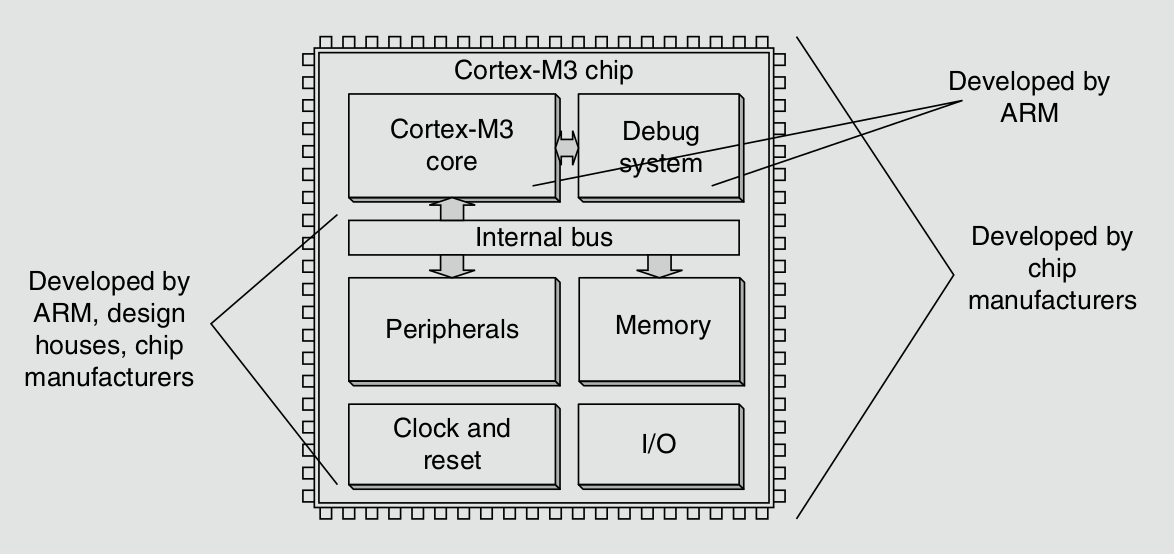
\includegraphics[width=0.6\textwidth]{arm_vs_custom_modules.png}
    \caption{Разбиение реализации подсистем процессора.}
\end{figure}


Процессор использует Гарвардскую архитектуру, имеется отдельная шина инструкций и шина данных. Однако шины инструкции и данных используют единое пространство памяти. Поэтому общая память системы делится между данными и инструкциями. Процессор Cortex-M3 включает в себя ряд фиксированных внутренних компонентов отладки которые разрабатываются компанией ARM. Эти компоненты обеспечивают поддержку операций отладки и функции, такие как точки останова (breakpoints) и точки наблюдения (watchpoints).

\begin{figure}[h!]
    \centering
    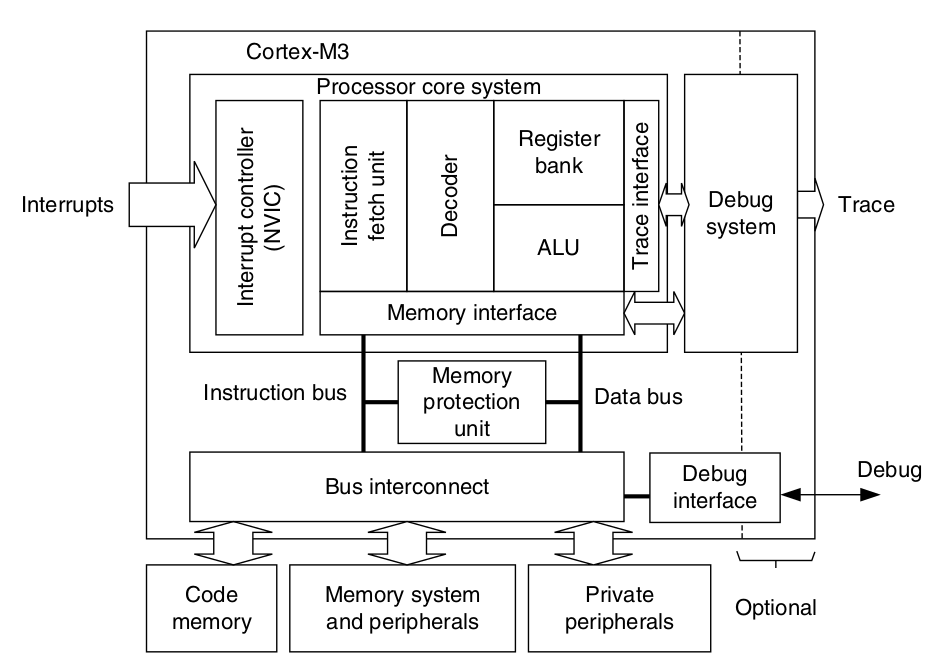
\includegraphics[width=0.6\textwidth]{cortex_m3_subsystems_overview.png}
    \caption{Подсистемы процессора Cortex-M3.}
\end{figure}


Функционал Trace отключен. Подсистема MPU (Memory Protection Unit) не поддерживается.
Процессор имеет два режима работы: Привилегированный и пользовательский режим. В данной работе используется только привилегированный режим. Cortex-M3 предоставляет стандартизированную схему разбиения адресов для разработчиков микроконтроллеров. Это важно для функционирования программы поскольку определяет способ для взаимодействия между программой на C и периферией процессора. В данном случае доступ к периферии производится обращением к определенным ячейкам памяти. Производители могут модифицировать схему разделов памяти. Как описано в разделе о границах RAM памяти Realtek немного модифицировал разбиения памяти. ROM память находится по адресам с 0х00000000 по 0х000FFFFF. SRAM расположена по адресам с 0х10000000 по 0х1006FFFF. Доступ к памяти SDRAM осуществляется по адресам с 0х30000000 по 0х301FFFFF.
 
\begin{figure}[h!]
    \centering
    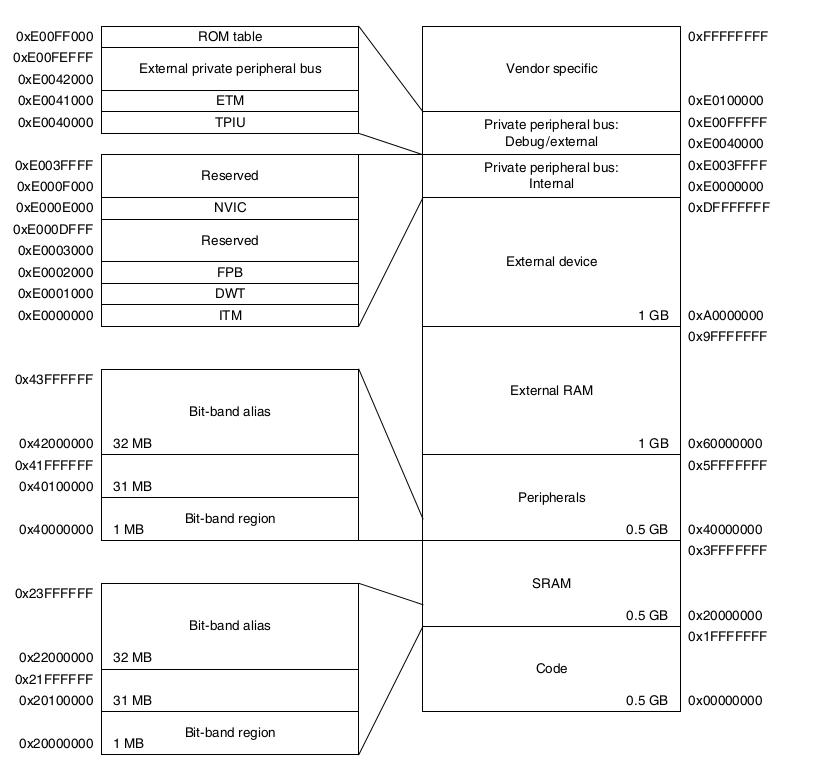
\includegraphics[width=0.9\textwidth]{predefined_memory_map.png}
    \caption{Разбиение памяти для микроконтроллера Cortex-M3.}
\end{figure}


Поддержка аппаратных прерываний осуществляется с помощью NVIC (Nested Vectored Interrupt Controller). Важными особенностями NVIC для функционирования программы являлось то что он поддерживает вектор прерываний (vectored interrupt support), вложенные прерывания на аппаратном уровне (nested interrupt support), программно устанавливаемые приоритеты для прерываний (dynamic priority changes support), маскировку прерываний (interrupt masking).


Процессор взаимодействует с периферией через несколько шин. Ниже представлена блок-схема подключения периферии включая шину для отладки внутри процессора.

\begin{figure}[h!]
    \centering
    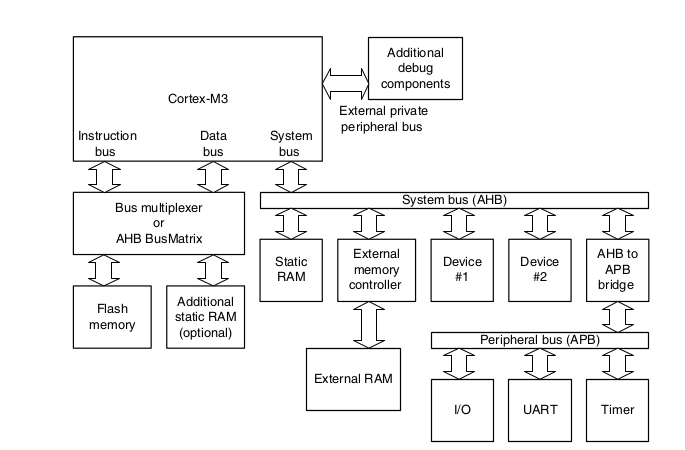
\includegraphics[width=0.8\textwidth]{cortex_m3_peripherals_block_diagram.png}
    \caption{Блок-схема подключения периферии к шинам внутри процессора.}
\end{figure}


Процессор Cortex-M3 включает в себя функции отладки. Поддерживает JTAG или SW (Serial-Wire) интерфейс для внешнего отладчика. Технология реализующая подсистему отладки процессора - CoreSight. С ее помощью можно получить доступ к состоянию регистров процессора и содержимому ячеек памяти. Есть встроенная поддержка шести точек останова (breakpoints) и четырех точек наблюдения (watchpoints). [CoreSight Technology System Design Guide]

В Cortex-M3, доступ к функционалу для отладки расположенному на процессоре осуществляется через интерфейс шины DAP (Debug Access Port). DAP управляется другим компонентом известным как DP (Debug Port) который преобразует команды JTAG или SW (Serial-Wire) поступающие из внешнего отладчика в команду DAP и направляет ее на шину. Ниже приведены схема подключения отладчика к процессору, а также  схема взаимодействия компонентов отладки Cortex-M3. 


\begin{figure}[h!]
    \centering
    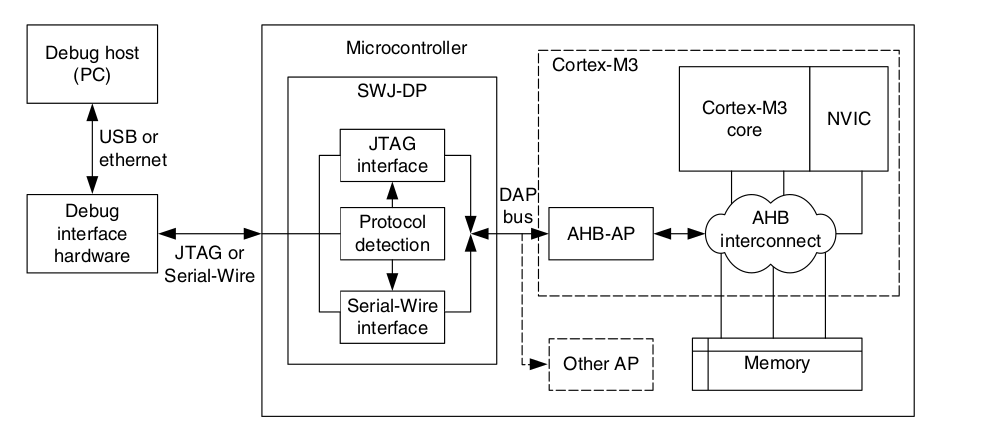
\includegraphics[width=0.9\textwidth]{cortex_m3_debug_connection.png}
    \caption{Схема подключения отладчика к процессору Cortex-M3.}
\end{figure}


\begin{figure}[h!]
    \centering
    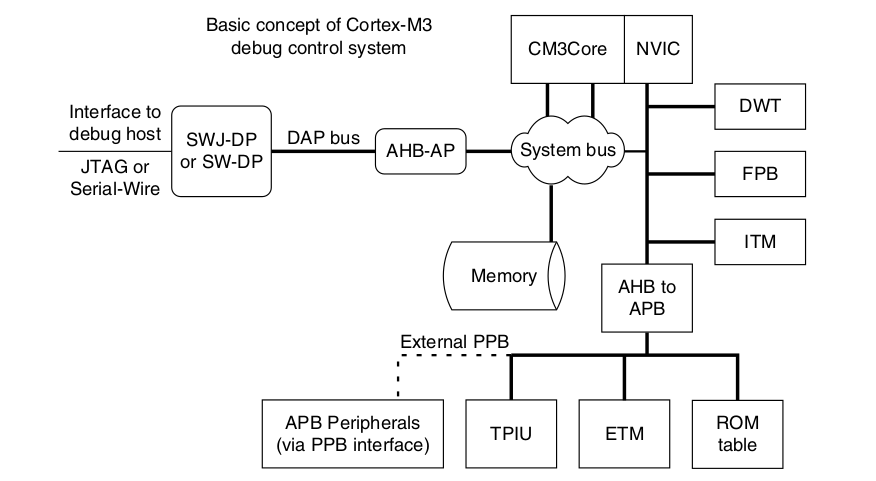
\includegraphics[width=0.9\textwidth]{cortex_m3_inside_debug_subsystem.png}
    \caption{Схема взаимодействия компонентов отладки Cortex-M3.}
\end{figure}

.


\newpage

\subsection{Платформа Браузер}
На самом деле не следует рассматривать конкретный браузер как платформу для разработки. Следует рассматривать набор спецификаций которые суммарно определяют веб-платформу. Браузер лишь реализует данные спецификации и предоставляет разработчику доступ к конкретной реализации веб-платформы.

\subsubsection{ Организации выпускающие спецификации веб-платформы}
Стандарты публикуемые организацией W3C определяют основные компоненты веб-платформы. Границы веб-платформы продолжают развиваться. Краеугольным камнем веб-платформы является HTML5, однако функционал используемый в данной работе зависит от многих других спецификаций, которые создают W3C и другие организации. В частности CSS, SVG, WOFF, ECMAScript и различные браузерные API.

В разработке спецификаций которые определяют веб-платформу участвуют несколько организаций. Ниже перечислены ключевые организации публикующие стандарты которые определяют веб-платформу.

\begin{my_enumerate}
\item Рекомендации, опубликованные консорциумом World Wide Web Consortium (W3C) [2], такие как HTML / XHTML, каскадные таблицы стилей (CSS), объектная модель документа (DOM), форматы изображений, такие как портативная сетевая графика (PNG) и масштабируемая векторная графика (SVG), а также специальные технологии, такие как WOFF.
\item Стандарты, опубликованные Ecma International (ранее ECMA) [4], такие как JavaScript (также известный как "стандартный ECMAScript")[3]
\item Стандарты, опубликованные международной организацией по стандартизации (ISO) [5], такие как JPEG.
\end{my_enumerate}


\subsubsection{ Спецификации определяющие веб-платформу}
Набор спецификаций определяющий веб-платформу позволяет разработчику абстрагироваться от конкретного браузера. Это существенно облегчает разработку веб-приложения которое должно работать в различных браузерах.

Когда веб-сайт или веб-приложение описываются как соответствующие стандартам веб-платформы или просто веб-стандартам, это означает, что сайт или приложение имеют допустимые стандартом HTML, CSS и JavaScript. HTML отвечает требованиям доступности для людей с нарушением зрения (дальнозоркостью или дальтонизмом) или движений, благодаря размещению специальных пометок и дополнительной информации на странице, а также другим семантическим рекомендациям. Полное соответствие стандарту охватывает также корректные параметры для кодирования символов, корректные метаданные, корректно сформированный XML, корректное встраивание скриптов и правильную настройку сервера.

Компонент программы который предназначен для исполнения в браузере, то есть для запуска на веб-платформе, требует для успешной работы чтобы браузер поддерживал следующие основополагающие спецификации описывающие веб-платформу.

\begin{my_enumerate}
\item Рекомендации для языков разметки, таких как язык разметки HTML (HyperText Markup Language) и масштабируемая векторная графика (Scalable Vector Graphics) из W3C.
\item Рекомендации для таблиц стилей, особенно каскадных таблиц стилей (Cascading Style Sheets), от W3C.
\item Стандарты для ECMAScript, чаще JavaScript, от Ecma International.
\item Рекомендации для объектных моделей документов (Document Object Model) от W3C.
\item Правильно сформированные имена и адреса для страницы и всех других ресурсов, на которые в ней есть ссылки (Uniform Resource Idenfirier), на основе RFC 2396, из IETF.[12]
\item Правильное использование HTTP и MIME типов для скачивания веб-страницы, ее интерпретации и запроса других ресурсов, упомянутых в ней, на основе RFC 2616, из IETF.[13]
\item Веб-доступность обычно основана на руководящих принципах доступности веб-контента[14], опубликованных инициативой W3C по веб-доступности.
\end{my_enumerate}

\subsubsection{ Реализация веб-платформы в различных браузерах}
При создании компонента программы для веб-платформы важно помнить что в итоге компонент должен будет запускаться на конкретной версии конкретного браузера на конкретном пользовательском устройстве (операционной системе).
Разработка компонента для браузера не тривиальна, в силу того что существует несколько популярных браузеров, у многих есть мобильные версии, у одного браузера есть несколько популярных устаревших версий браузера, и наконец для каждой операционной системы существует своя версия браузера. Каждая из этих мобильных или десктопных версий является своей обособленной реализацией веб-платформы. Каждая из этих мобильных или десктопных версий имеет свои уникальные ошибки и баги в реализации стандартов описывающих веб-платформу. Веб-разработчик сталкивается с проблемами дырявых абстракций (leaky abstractions)[https://www.joelonsoftware.com/2002/11/11/the-law-of-leaky-abstractions/] в том как браузеры реализуют стандарты описывающие веб-платформу.


\subsubsection{ Поддерживаемые браузеры}
Из-за большого количества различных реализаций веб-платформы невозможно вести разработку нацеленную на правильную работу во всех браузерах. Необходимо выделить реальное подмножество на которое будет нацелена разработка из множества всех комбинаций версий, типов браузеров и версий, типов операционных систем.

При разработке компонента для запуска в браузере следует учитывать что после его интеграции в программу для управления и мониторинга РВ-90 у разработчика не будет возможности что-либо изменить в данном компоненте. В силу данного факта следует уделить уделить особое внимание правильному пониманию и использованию стандартов описывающих веб-платформу, а также следует стремиться максимально расширить множество поддерживаемых браузеров, чтобы охватить как можно больше наиболее распространенных версий.

Следует определить каким именно браузерам стоит уделить внимание при разработке. 
Для данной программы было решено ограничиться поддержкой браузеров которые имеют более 0.05\% рынка пользователей в России, при этом исключив из этого списка браузеры Internet Explorer версии 9 и раньше, а также браузер Opera mini. Для определения конкретных версий и названий браузеров, которые должны стать ключевыми при реализации были использованы проекты "Can i use" и "Browserlist".

Также не представлялось возможным осуществить поддержку каждой из всех 30 распространенных версий Gogole Chome и Firefox поэтому для тестирования были выбраны самые новые и самые старые из популярных версий каждого браузера.
Ниже приведен итоговый список поддерживаемых браузеров для программы управления и контроля РВ-90.

\textbf{Мобильные браузеры}
\begin{my_itemize}
\item Chrome for Android 73
\item Firefox for Android 66
\item UC Browser for Android 11.8
\item Android Browser 4.4
\item Android Browser 4
\item IE Mobile 11
\item iOS Safari 12
\item iOS Safari 8
\item Samsung Internet 9.2
\item Samsung Internet 7
\end{my_itemize}

\textbf{Десктопные браузеры}
\begin{my_itemize}
\item Chrome 74
\item Chrome 52
\item Firefox 66
\item Firefox 48
\item Edge 18
\item IE 10
\item Opera 58
\item Opera 39
\item Safari 12
\item Safari 9
\end{my_itemize}

С аппаратной точки зрения также следует помнить что размер окна браузера меняется в зависимости от настроек пользователя. Поэтому компонент должен поддерживать адаптивный интерфейс  корректно работающий при разных размерах экрана.  На данный момент браузеры на других платформах как например умные часы или умный телевизор не являются официально поддерживаемыми. Приведенные выше браузеры являются поддерживаемыми платформами для работы одно-страничного веб-приложения являющимся одним из трех компонентов программы для управления РВ-90.


\newpage
\subsection{Платформа Android}
Приложения для платформы Android запускаются в виртуальной машине Java, которая предоставляет абстракцию от аппаратной базы устройства.

Android предназначен для работы на различных видах устройств, от телефонов до планшетов и телевизоров. 
Приложение для Android гарантированно совместимо со всеми устройствами Android, однако может быть не совместимо с конкретной конфигурацией устройства. Например, некоторые устройства могут не иметь  Wi-Fi соединения. Если основные функции приложения требуют использования наличие Wi-Fi соединения, приложение совместимо только с устройствами, которые имеют возможность устанавливать соединение по сети Wi-Fi. Приложение может быть совместимо с телефоном и планшетом, но не совместимо с умным телевизором.
Android предоставляет возможность создать отдельный APK (Android Package) для различных конфигураций устройства. В рамках данной работы планируется разрабатывать только один APK (Android Package) который будет удовлетворять конфигурациям наибольшего количества устройств. 

Компонент программы предназначенный для работы на платформе Android, должен работать лишь на планшетах и телефонах. С точки зрения реализации отличие планшетов от телефонов заключается лишь в разных конфигурациях экрана.

Ниже перечислены параметры конфигурации приложения которые влияют на ограничение доступности приложения для устройств через Google Play Store.  
Соответственно данные параметры определяют более конкретную конфигурацию для платформы Android на которой будет запускаться третий компонент программы.

\begin{my_enumerate}
\item Особенности устройства
\item Версия платформы
\item Конфигурация экрана
\end{my_enumerate}

\subsubsection{Особенности устройства}
Чтобы управлять доступностью приложения на основе функционала самого устройства, Android определяет идентификаторы функций для любого оборудования или программного обеспечения, которые могут быть недоступны на устройствах. Например, идентификатор функции для датчика компаса - FEATURE\_SENSOR\_COMPASS, а идентификатор функции для виджетов приложений-FEATURE\_APP\_WIDGETS.
При необходимости можно запретить пользователям установку приложения, если их устройства не предоставляют данную функцию, объявив ее с элементом <uses-feature> в файле манифеста приложения.
Компонент для Android не требует наличия нестандартной функциональности, поэтому проект не пользуется данным ограничением.

\subsubsection{Версия платформы}
На разных устройствах могут работать разные версии платформы Android, такие как Android 4.0 или Android 4.4. Каждая последующая версия платформы часто добавляет новые API, недоступные в предыдущей версии. Чтобы указать, какой набор API, каждая версия платформы задает уровень API. Например, Android 1.0-это уровень API 1, а Android 4.4-уровень API 19.
Уровень API позволяет объявить минимальную версию, с которой совместимо приложение, используя тег манифеста <uses-sdk> и его атрибут minSdkVersion. Например, API поставщика календаря были добавлены в Android 4.0 (уровень API 14). Если приложение не может работать без этих API, следует объявить уровень API 14 минимальной поддерживаемой версией приложения.

Атрибут minSdkVersion объявляет минимальную версию, с которой совместимо приложение, а атрибут targetSdkVersion объявляет самую высокую версию, на которой оптимизировано приложение.
Для реализации данного компонента была выбрана настройка minSdkVersion = 15, а targetSdkVersion = 22. Данные настройки для минимальной версии SDK гарантируют что приложение будет работать на более чем 95\% процентах устройств подключающихся к Google Play Store. targetSdkVersion намеренно выставлено столь низко чтобы обойти проблему динамического запроса разрешений пользователя на использование определенных API, вместо этого запрос на разрешение выполняется в процессе установки приложения из Google Play Store [\url{https://developer.android.com/guide/topics/permissions/overview#install-time_requests_android_511_and_below}].

\subsubsection{Конфигурация экрана}
Android работает на устройствах различных размеров, от телефонов до планшетов и телевизоров. Чтобы классифицировать устройства по типу экрана, Android определяет две характеристики для каждого устройства: размер экрана (физический размер экрана) и плотность экрана (физическая плотность пикселей на экране, известная как DPI или Dots Per Inch). Чтобы упростить различные конфигурации, Android обобщает эти варианты в группы, которые облегчают их использование.

Четыре обобщенных размера: 
\begin{my_enumerate}
\item small (маленький)
\item normal (нормальный)
\item large (большой)
\item xlarge (очень большой)
\end{my_enumerate}

И несколько обобщенных плотностей: 
\begin{my_enumerate}
\item mdpi (средняя)
\item hdpi (высокая)
\item xhdpi (очень высокая)
\item xxhdpi (экстра-экстра высокая)
\end{my_enumerate}

По умолчанию приложение совместимо со всеми размерами и плотностями экрана, поскольку система вносит необходимые изменения в макет пользовательского интерфейса и ресурсы изображений по мере необходимости для каждого экрана.

В данной работе компонент никак не ограничивает ни размер, ни плотность экрана.



%===========================================================================



\newpage
\subsection{Архитектура прошивки для РВ-90}
% what is it
% what it does
Прошивкой является файл типа .bin который прошивается во флеш-память находящуюся на модуле RAK473.

Прошивка осуществляет контроль за периферией реле и является основным компонентом программы.

Ниже изображена блок схема компонент прошивки, на которой отражены активные потоки системы. Каждая пользовательская библиотека и поток представляют собой отдельный модуль системы. На диаграмме разбиение на пользовательские и системные модули, разделяет модули которые поставлялись в комплекте с SDK от модулей которые реализованы в данной работе.

\begin{figure}[h!]
    \centering
    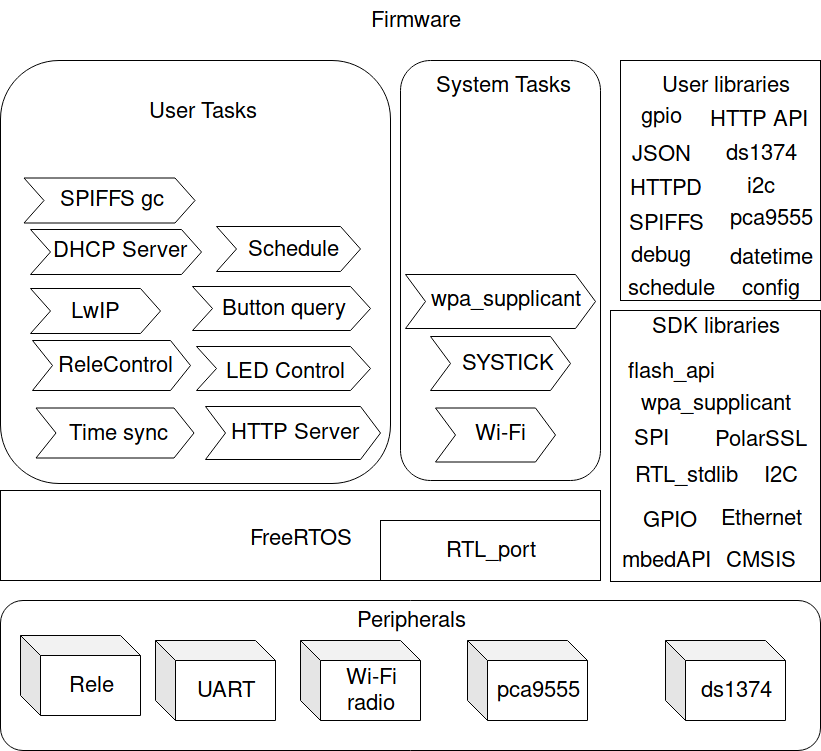
\includegraphics[width=0.9\textwidth]{firmware_modules_diagram.png}
    \caption{Блок схема отображающая модули прошивки.}
\end{figure}

Для организации работы используются потоки FreeRTOS. Поток - это абстракция предоставляемая FreeRTOS, которая используется для организации работы системы и контроля за доступам к ресурсам и периферии системы. Каждый поток предельно прост и призван выполнять только одну функцию, однако самих потоков довольно много. Чтобы модули потоков были наиболее просты для понимания и поддержки, как можно больший пласт функций находится в пользовательских библиотеках, которые выделены в отдельные модули. В результате данной архитектуры в системе есть много простых потоков которые используют сложные схемы для синхронизации и взаимодействия. Все потоки кроме потока LwIP работают по схеме: проснуться, проверить наличие работы, поработать, поставить таймер и заснуть на некоторый интервал времени. Поток LwIP является потоком по умолчанию который работает когда все остальные задачи спят. Потоки взаимодействуют друг с другом через примитивы синхронизации, а именно семафоры и очереди.

В частности прошивка создает и поддерживает точку доступа к сети Wi-Fi. Что снижает риск безопасности, связанный с распространением информации через Интернет. 
Прошивка устанавливается на РВ-90 при производстве устройства. Код входящий в прошивку разбит на несколько модулей. Модули разделены на основе функциональности, которая должна присутствовать в реле времени.


\subsubsection{ Прошивка для РВ-90 }
Файл прошивки получается на последнем этапе компиляции, посредством обработки EFL (Executable and Linkable Format, Extensible Linking Format) файла программы. 
Файл Bin - это чистый двоичный файл без исправлений памяти или перемещений, он требует загрузки по определенному адресу памяти.
Файлы ELF - это более сложный формат, состоящий из секций не все из которых предназначены для загрузки в RAM память. Формат включает в себя таблиц для поиска символов и таблицы перемещений. Он предназначается для загрузки операционной системой по произвольному адресу памяти, адреса переменных в этом случае вычисляются во время выполнения используя таблицу GOT (Global Offset Table). 

Ниже представлена схема сборки прошивки с помощью официального SDK от Realtek и GNU GCC ARM Toolchain.
 
\begin{figure}[h!]
    \centering
    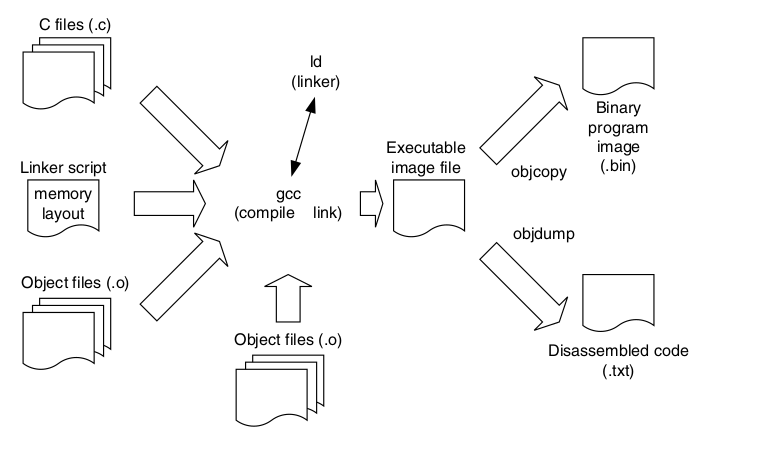
\includegraphics[width=0.7\textwidth]{compilation_steps_firmware.png}
    \caption{Этапы сборки прошивки РВ-90.}
\end{figure}

К данному процессу стоит добавить этап после получения .bin файла, а именно сборку образа файловой системы в которой хранится веб-компонент программы. А также объединение образа файловой системы и прошивки в единый образ прошивки. 


\begin{figure}[h!]
    \centering
    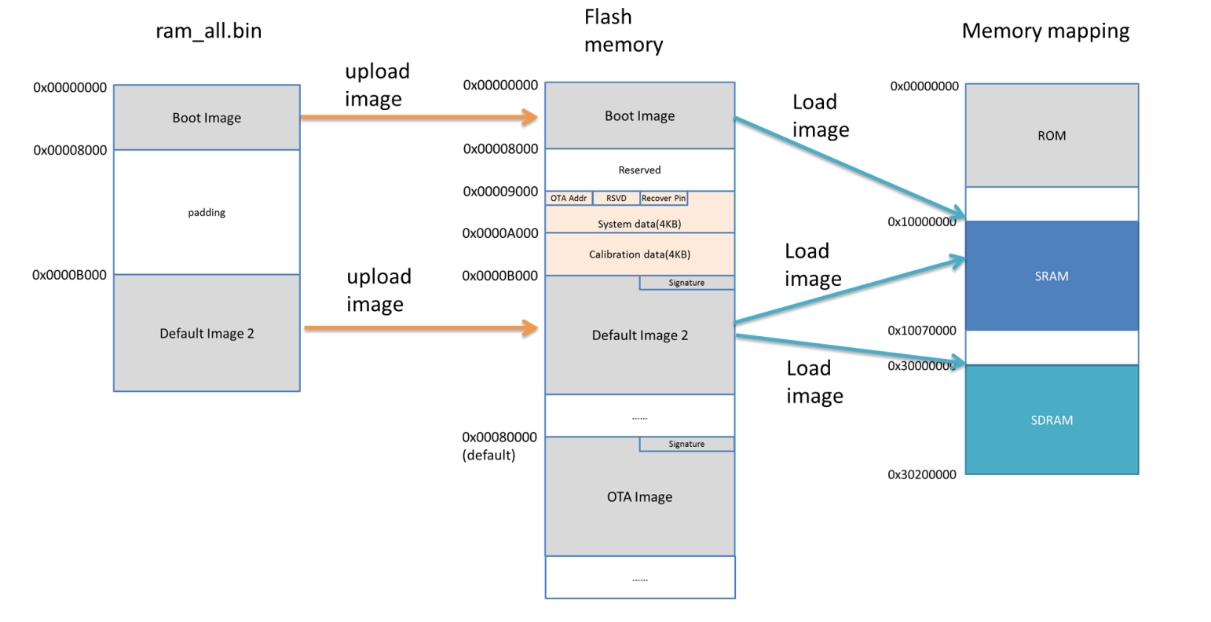
\includegraphics[width=1.0\textwidth]{from_firmware_to_ram.png}
    \caption{Код в файле прошивки, во флеш-памяти и наконец при загрузке в RAM.}
\end{figure}


\subsubsection{ Описание архитектуры модулей}
Для организации работы и разделения ресурсов периферии используется модуль FreeRTOS. 
FreeRTOS - предоставляет ядро операционной системы реального времени для встроенных устройств. FreeRTOS разработан с целью создания простой и компактной в плане использования RAM операционной системы. Само ядро состоит только из трех C-файлов. Чтобы сделать код читаемым, легко портируемым и поддерживаемым, он написан в основном на C, но там, где это необходимо, есть несколько ассемблерных функций (в основном в подпрограммах для планировщика архитектуры).

FreeRTOS предоставляет методы для создания потоков (task), примитивов синхронизации, таких как мьютекс (mutex), семафор (semaphore), а также программных таймеров. Потокам можно назначать разные приоритеты. FreeRTOS предоставляет свой аллокатор памяти, объекты RTOS могут быть динамически распределены с помощью пяти схем выделения памяти:

\begin{my_enumerate}
\item heap\_1 - самая простая, не позволяет освобождать память.
\item heap\_2 - позволяет освободить память, но не производит объединения соседних свободных блоков.
\item heap\_3 - обертка вокруг стандартных malloc() и free() для безопасности обращения из потоков.
\item heap\_4 - производит объединения соседних свободных блоков чтобы избежать фрагментации.
\item heap\_5 - также как и heap\_4, с возможностью работать с heap который распределен на нескольких не смежных областей памяти.
\end{my_enumerate}

Модуль для управления выходом реле (включено-выключено).
Данный модуль периодически проверяет очередь событий и если в ней есть событие на включение или выключение реле, то модуль приводит его в действие. Для этого он запрашивает доступ к I2C шине и передает команду I2C расширителю портов PCA9555 на выключение или включение пина к которому подключено одно из двух реле. Для определения номера необходимого пина модуль обращается к модулю config. 

Модуль для TCP/IP потока LwIP. Он ждет приходящих пакетов на ранее зарегистрированный интерфейс, или просматривает очередь на наличие пакетов ожидающих отправки через определенный ранее зарегистрированный интерфейс.

Модуль управления DHCP сервером получает DHCP пакеты от модуля TCP/IP потока LwIP, обрабатывает их и выдает ответ. Модуль следит за набором доступных IP адресов.

Модуль управления HTTP сервером получает HTTP запросы от модуля TCP/IP потока LwIP, интерпретирует их с помощью модуля HTTPD, обрабатывает их и либо обращается к модулю HTTP API для генерирования ответа, либо обращается к модулю SPIFFS для передачи в ответ на запрос файла из файловой системы. 

Модуль вывода отладочной информации.
Предоставляет набор функций и макросов для контроля над дебаг информацией передаваемой по UART.

Модуль для генерации ответа HTTP API предоставляет набор шаблонов для генерации стандартных ответов HTTP сервера. Также модуль может обращаться к файловой системе для чтения или записи новых настроек поступивших от пользователя, и к модулю генерации и интерпретации JSON для работы с запросами.

Модуль для анализа и генерации JSON.
Предоставляет функции для интерпретации и генерации JSON строки из переменных языка C.

Модуль для управления коммуникацией по протоколу I2C, предоставляет альтернативную реализацию протокола I2C вместо неправильно реализованной версии в официальном SDK от Realtek.

Модуль для связи с чипом DS1307 предоставляет набор команд для настройки и чтения текущего времени, а также для настройки таймера аппаратного прерывания, расположенного в чипе DS1374. Все взаимодействие происходит через протокол I2C.

Модуль управления временем системы раз в час синхронизирует внутренний счетчик системы со счетчиком расположенным в DS1374.

Модуль управления файловой системой предоставляет доступ к чтению и записи файлов файловой системы, одновременно предоставляя защиту от одновременного доступа нескольких потоков. 


\subsubsection{ Официальный SDK от Realtek}
На самом деле сложно разграничить официальный SDK от пользовательского кода, т.к. при сборке проекта обе части собираются вместе.
Между кодом SDK и пользовательским кодом образуется взаимосвязь, так как некоторые аспекты платформы приходится настраивать в самом SDK.

SDK имеет сравнительно мало закрытых бинарных библиотек. Многие закрытые функции содержаться в ROM памяти микроконтроллера. 
При соотношении полученных на выходе команд ассемблера можно сказать что 70\% SDK это открытый исходный код. Наличие большого объема открытого кода позволяет существенно уменьшить SDK при этом не теряя функциональности для программы управления РВ-90.   

Официальный SDK имеет довольно запутанную структуру. Причина отчасти в том что SDK поддерживает одновременно две различных аппаратных платформы Ameba-Zero и Ameba-One. Ameba - это название аппаратной платформы для разработки решений в сфере IoT (Internet of Things) от компании Realtek. Ameba-Zero использует микроконтроллер RTL8710. Аmeba-One использует микроконтроллер RTL8195 который совместим с микроконтроллером RTL8711AM, но предоставляет больше функций.

Для упрощения работы с SDK из него были выкинуты файлы использующиеся лишь при сборки проектов Ameba-Zero.


\subsubsection{ Разбор кода предоставляемого компанией ARM}
Вместе с ядром ARM предоставляет стандарт CMSIS  (Cortex Microcontroller Software Interface Standard).
CMSIS предоставляет интерфейс на языке C который реализуется производителями микроконтроллеров, в частности компанией Realtek, для предоставления доступа из языка С к определенным функциям, которые есть на всех процессорах Cortex-M. Для программы контроля и управления РВ-90, важно что данный интерфейс предоставляет функции для доступа к регистрам, NVIC, определения частоты процессора.

Вместе с ядром ARM также предоставляет стандарт Mbed API.
Mbed - это набор библиотек для упрощения разработки подключенных к интернету устройств на базе 32-разрядных микроконтроллеров ARM Cortex-M. Проект совместно разрабатывается ARM, партнерами и волонтерами от сообщества mbed. Код разрабатывается под лицензией Apache 2.0. Он включает в себя все основные программные компоненты для встроенных систем, такие как операционную систему, TCP/IP стек, а также множество портов HAL (Hardware Abstraction Layer), которые позволяют mbed работать на микроконтроллерах с ядром Cortex-M от разных производителей практически без изменения пользовательского кода.
Mbed предоставляет интерфейс на языке C который реализуется производителями микроконтроллеров, в частности компанией Realtek, для предоставления доступа из языка С к периферии микроконтроллера, а также к большому набору функций описанных в спецификации Mbed API, таких как реализация ОС и TCP/IP стека. 

Mbed API в данной работе не используется. Вместо этого для контроля периферии напрямую используются функции предоставляемые компанией Realtek. Mbed предоставляет дополнительный уровень абстракции поверх FreeRTOS и LwIP. Вместо того чтобы использовать данный уровень абстракции, обращение к функционалы FreeRTOS и LwIP происходит напрямую. Это сделано чтобы существенно уменьшить размер прошивки на флеш-памяти и при загрузке в RAM, позволяя освободить память для файлов веб-компонента и пользовательских настроек. 


\newpage
\subsection{Архитектура одно-страничного веб-приложения для браузера}
% what is it
% what it does
Одно-страничное веб-приложение храниться во флеш-памяти микроконтроллера в виде набора файлов и передается на подключенное устройство пользователя когда пользователь инициирует запрос корневого документа.

Пользовательский интерфейс к реле реализован в веб-приложении. Веб-приложение позволяет пользователю отследить и изменить состояние реле. Включая изменение состояния, контактов, изменение названия и пароля Wi-Fi сети, изменение текущего времени системы. Также веб-приложение позволяет пользователю составить программу включений и выключений на 2 года вперед, и передает данную программу на РВ-90.

Архитектура для веб-приложения предельно проста. Корневой файл index.html предоставляет все элементы которыми будут манипулировать Javascript и CSS модули. Два модуля constants.js и globals.js используются для объединения DOM описанном в index.html с другими модулями. Три модуля CSS определяют вид приложения.

\begin{figure}[h!]
    \centering
    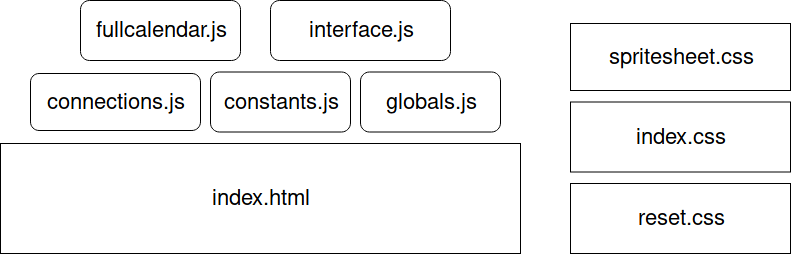
\includegraphics[width=0.9\textwidth]{webapp_modules_blocks.png}
    \caption{Блок схема отображающая модули одно-страничного веб-приложения.}
\end{figure}

\subsubsection{ Загрузка и запуск компонента}
При подключении пользователь запрашивает корневой файл, в ответ HTTP сервер возвращает index.html
Вместе с ним загружается основной файл стилей CSS и Javascript модуль connections.js для динамической подгруздки в бекграунд процессе остальных файлов. Остальными файлами являются дополнительные стили CSS и модули Javascript содержащие функции манипулирования DOM в index.html, и в частности модуль для создания расписания включений и выключений fullcalendar.js  

\subsubsection{ Кросс-браузерное тестирование}
Веб-разработчик сталкивается с проблемами дырявых абстракций (leaky abstractions)[https://www.joelonsoftware.com/2002/11/11/the-law-of-leaky-abstractions/] в том как браузеры реализуют стандарты описывающие веб-платформу, поэтому при реализации требуется проводить кросс-браузерное тестирование.
Разработка и тестирование компонента для браузера не тривиальна, в силу того что 
существует несколько популярных браузеров, у многих есть мобильные версии, у одного браузера есть несколько популярных версий браузера, для каждой операционной системы существует своя версия браузера. Каждая из этих мобильных или десктопных версий является своей обособленной реализацией веб-платформы. Каждая из этих мобильных или десктопных версий имеет свои уникальные ошибки и баги в реализации стандартов описывающих веб-платформу. 

Из-за большого количества различных реализаций веб-платформы в браузерах кросс-браузерное тестирование на реальных комбинациях версий, типов и операционных систем является необходимым этапом разработки. При разработке компонента для запуска в браузере следует учитывать что после его интеграции в программу для управления и мониторинга РВ-90 у разработчика не будет возможности что-либо изменить в данном компоненте. Поэтому при разработке компонента для исполнения в браузере следует уделить особое внимание правильному пониманию и использованию стандартов описывающих веб-платформу, а также кросс-браузерному тестированию. 

\subsubsection{ Описание архитектуры модулей}
Веб-приложение можно разложить на следующие модули.

Модуль для взаимодействия с сервером через AJAX подгружает в бекграунде дополнительные CSS и Javascript модули, а также предоставляет простой интерфейс для отправки запросов к серверу и получению ответов. Интерфейс основан на   (callbacks).

Модуль для отображения состояния реле показывает текущее состояние внутренних параметров РВ-90. Модуль также следит за своевременным и консистентным обновлением веб-интерфейса.

Модуль для настройки включений и выключений реле предоставляет тот же функционал который можно встретить в других электронных реле времени. Оператор может: создать новый цикл включения/выключения и дать ему имя, назначить цикл определенному дню и установить его на повторение еженедельно или ежемесячно, установить исключения и переопределить циклы в определенные дни, получить обзор того, какие циклы выполняются в какие дни. Интерфейс интуитивно понятен и прост в использовании.

Модуль constants.js  содержит настройки для веб-приложения.

Модуль reset.css содержит инструкции для того чтобы привести стили которые браузеры выставляют по умолчанию к единому знаменателю.

Модуль index.css непропорционально велик по сравнению с другими CSS модулями, однако он содержит фактически все стили необходимые для правильной рисовки страницы.

Модуль spritesheet.css содержит координаты для каждой иконки в обшей карте иконок.


\newpage
\subsection{Архитектура мобильного приложения для Android}
% what is it
% what it does
Мобильное приложение представляет собой APK (Android Package) файл. Потенциально приложение может быть размещено в Google Play Store и доступно для установки на устройства Android.

Приложение позволяет предоставить пользователям более обширный функционал по сравнению с одно-страничным веб-приложением, за счет того что приложение позволяет более тесное взаимодействие с системой чем браузер. В частности приложение не имеет существенного ограничения по размеру устанавливаемого файла, в отличие от веб-интерфейса.

На данном этапе приложение предоставляет более удобный и дружелюбный для пользователя интерфейс создания календаря включений и выключений. Приложение является полностью опциональным компонентом системы и пользователю не требуется устанавливать его для того чтобы эксплуатировать реле по назначению.

Ниже представлена блок схема модулей приложения.



\subsubsection{ Описание архитектуры модулей}
Все модули приложения можно отнести к одной из 4 групп. Модули из группы Activity отвечают за различные экраны приложения, рисовку и логику взаимодействия элементов интерфейса. Модули из группы Controls реализуют новые элементы интерфейса для платформы Android которых не хватает в стандартной библиотеке. Модули из группы Netrowking отвечают за соединение с сервером РВ-90, сериализацию/десериализацию и прием/передачу данных. Наконец модули из группы DataModel реализуют бизнес сущности, то есть календарь (Calendar) состоит из циклов (Cycle), цикл состоит из временных отрезков (Timestrip). 
Ниже представлена блок схема модулей приложения.

\begin{figure}[h!]
    \centering
    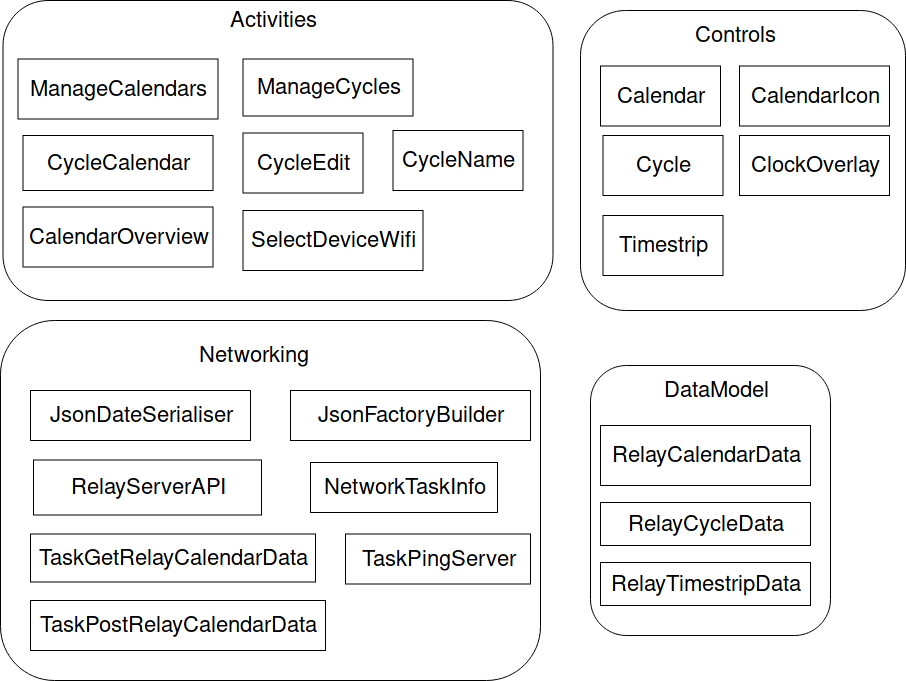
\includegraphics[width=0.9\textwidth]{mobile_module_blocks.png}
    \caption{Блок схема модулей приложения.}
\end{figure}

Нижеследующие модули реализуют какой либо экран приложения используя Activity. 
MainApplication открывается первым при запуске приложения. 
CalendarOverviewActivity позволяет пользователю просмотреть календарь на один год с возможностью точно видеть какой цикл запускается в какие дни.
CycleCalendarActivity позволяет пользователю посмотреть в какие дни работает конкретный цикл.
CycleEditActivity позволяет пользователю редактировать временные отрезки включения и выключения одного цикла.
CycleNameActivity позволяет пользователю задать для цикла название и цвет для отображения на календаре.
ManageCalendarsActivity позволяет пользователю создавать и удалять календари.
ManageCyclesActivity позволяет пользователю создавать и удалять циклы. Циклы не привязываются к календарю при создании.
SelectDeviceWifiActivity позволяет пользователю настроить Wi-Fi соединение с РВ-90.

Нижеследующие модули реализуют новые элементы интерфейса которые необходимы для приложения и которых нет в стандартной библиотеке Android.  
CalendarControl реализует элемент для компактного отображения календаря на один год.
CalendarIconControl реализует элемент для отображения иконки календаря.
ClockOverlay реализует элемент для отображения цикла и временных отрезков.
CycleControl реализует элемент совмещающий отображение циклов с отображением названия и цвета цикла.
TimeStripControl реализует элемент для отображения и редактирования временного отрезка.

Нижеследующие модули реализуют функционал для взаимодействия с HTTP сервером.  
GsonDateSerializer сериализует тип Datetime в строку формата JSON, т.к. по умолчанию данный тип не имеет представления в JSON формате.
GsonFactoryBuilder создает инстанцию для сериализации и десериализации JSON в соответствии с пользовательскими настройками.
NetworkTaskInfo содержит информацию для подключения к РВ-90. 
RelayServerAPI содержит декларативное описание HTTP API.
TaskGetRelayCalendarData реализует запрос HTTP GET для информации о календаре и циклах.
TaskPingServer реализует запрос на проверку соединения.
TaskPostRelayCalendarData реализует запрос HTTP POST на загрузку новых настроек в РВ-90.




%===========================================================================



\newpage
\subsection{Взаимодействие между модулями прошивки}
Диаграмма ниже показывает какие модули знают о каких других модулях. Если модуль является библиотекой, как например в случае с модулем JSON, то обращение к нему будет приходить через вызов функции. Иначе, если модуль является потоком, то обращение к нему будет происходить через примитивы синхронизации, то есть через семафор или очередь.

\begin{figure}[h!]
    \centering
    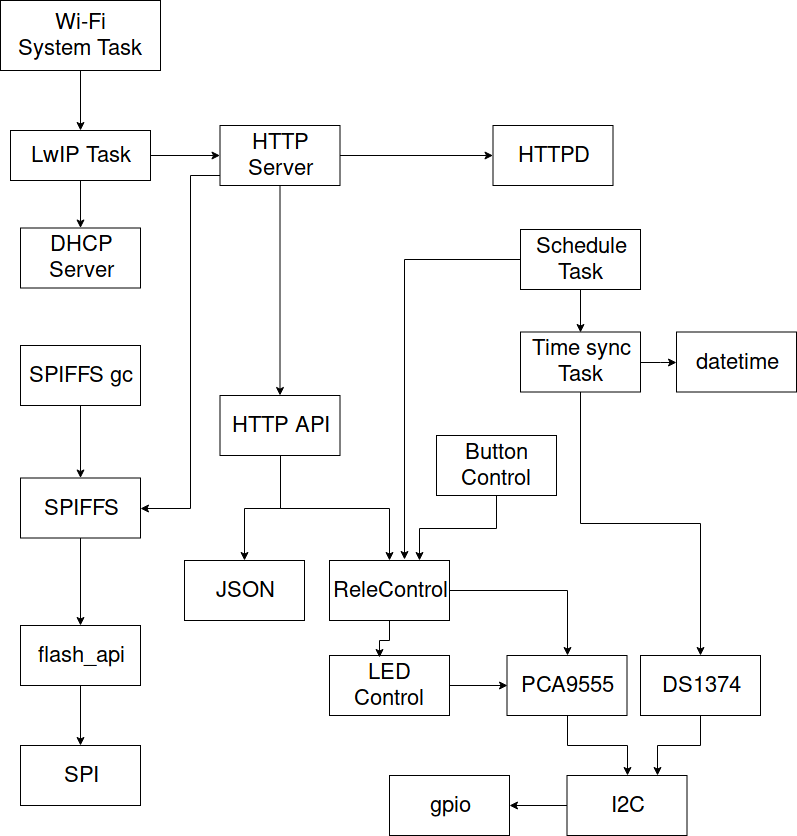
\includegraphics[width=0.7\textwidth]{firmware_module_hierarchy.png}
    \caption{Взаимодействие между модулями прошивки.}
\end{figure}


\newpage
\subsection{Взаимодействие между модулями одно-страничного веб-приложения}
Диаграмма ниже показывает какие модули знают и используют функционал объявленный в других модулях. В данной компоненте не принимались меры по ограничению взаимодействия между модулями. Каждому модулю доступны все объявления функций и переменных в том модуле с которым он связывается.

\begin{figure}[h!]
    \centering
    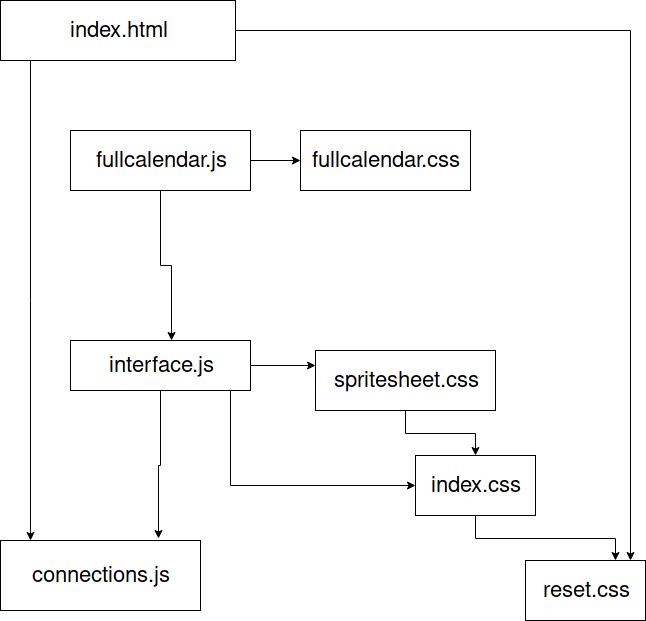
\includegraphics[width=0.7\textwidth]{webapp_modules_hierarchy.png}
    \caption{Взаимодействие между модулями одно-страничного веб-приложения.}
\end{figure}


\newpage
\subsection{Взаимодействие между модулями мобильного приложения}
Диаграмма ниже показывает какие модули знают и используют функционал объявленный в других модулях. В рамках Android модули общаются либо прямым вызовом функций либо через запуск Intent.

\begin{figure}[h!]
    \centering
    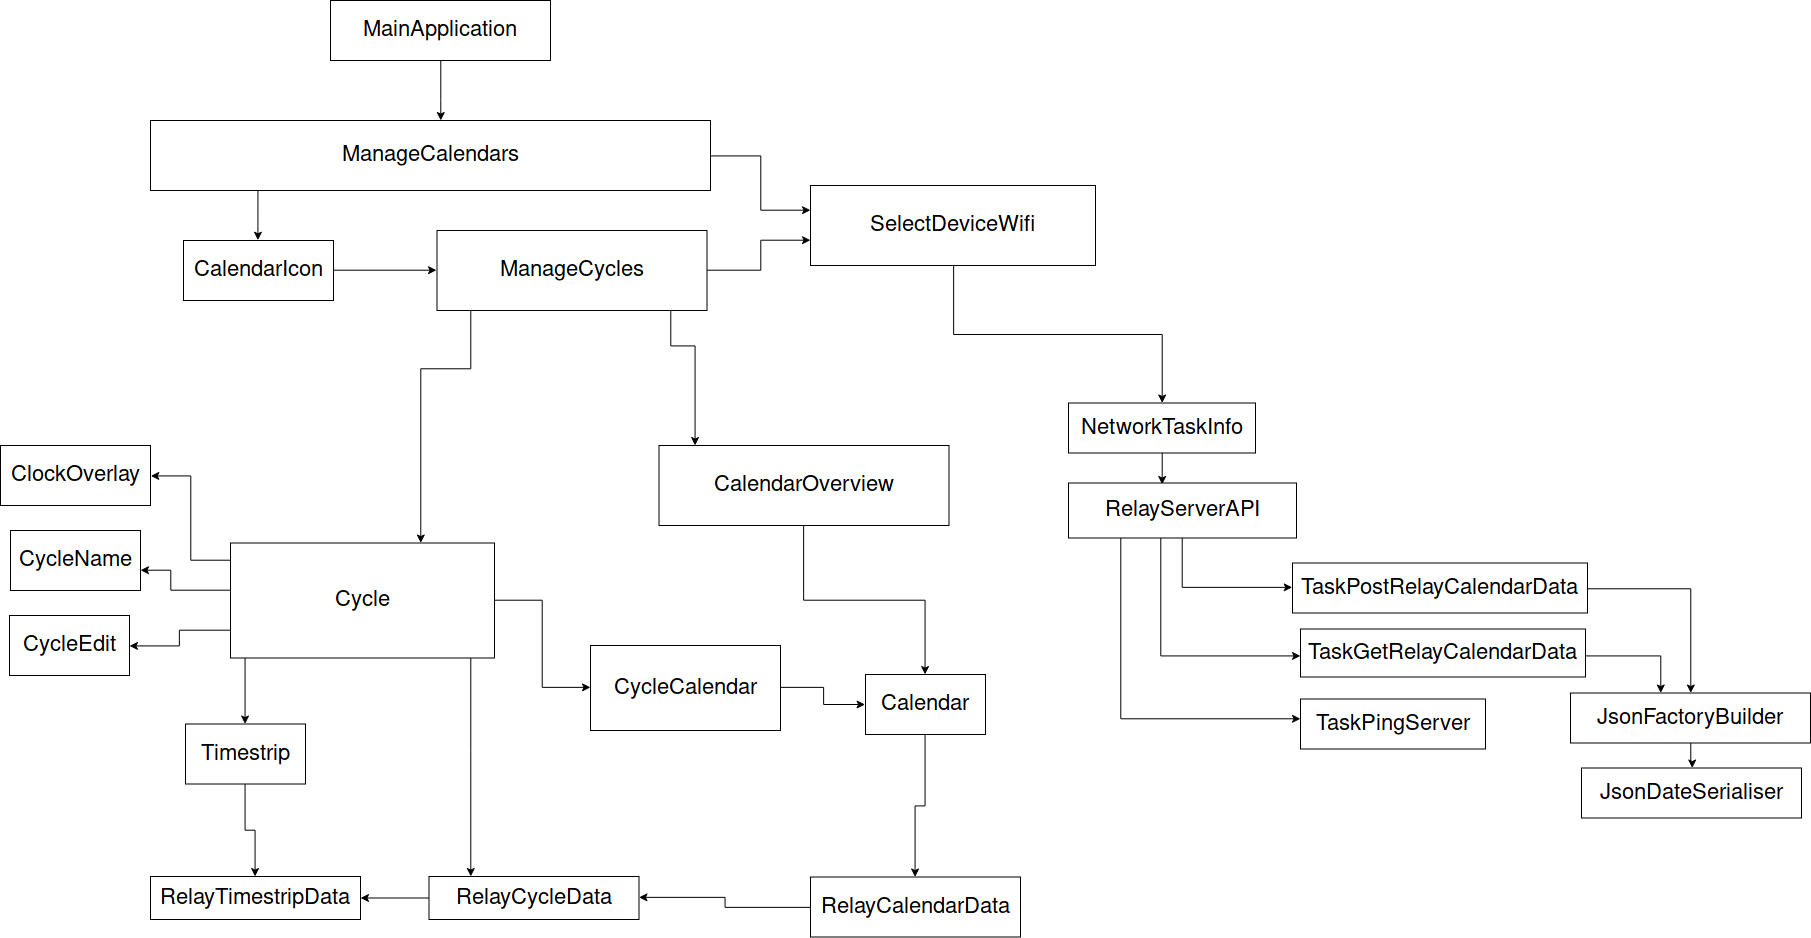
\includegraphics[width=1.03\textwidth]{mobile_modules_hierarchy.png}
    \caption{Взаимодействие между модулями мобильного приложения.}
\end{figure}


%===========================================================================


\newpage
\subsection{Взаимодействие между тремя компонентами программы}
Центральным компонентом является прошивка РВ-90. Она создает точку доступа и запускает HTTP сервер. Веб-приложение и мобильное приложение взаимодействуют с сервером.
Веб-приложение может либо обращаться к HTTP API, либо запрашивать файлы из файловой системы расположенной на флеш-памяти модуля RAK473. Мобильное приложение использует только HTTP API, т.к. вся информация для отображения интерфейса предоставляется вместе с APK.
HTTP API поддерживает несколько типов запросов. Планировалось сделать данное API как можно проще, чтобы избежать проблем с рассинхронизацией состояния между РВ-90 и тем состоянием которое отображается на устройстве пользователя. Самой частый вызов к API это "GET /read" который возвращает текущее состояние системы, а именно состояние контактов реле, текущее время, время следующего срабатывания для каждого реле, код состояния чипа реального времени, название сети Wi-Fi, пароль сети Wi-Fi, количество устройств подключенных к сети Wi-Fi на данный момент, состояние управления реле (ручное или автоматическое). Также присутствует "POST /set" принимающий запрос аналогичный "/read" но с желаемыми значениями. Также для того чтобы уменьшить нагрузку на Wi-Fi канал и уменьшить объем используемой RAM памяти для приема и передачи календаря, циклов, и временных отрезков используется не JSON, а бинарный формат.



%===========================================================================


\newpage
\subsection{Выводы по главе}
Разобрана общая трехкомпонентная архитектура программы. С аппаратной точки зрения описаны платформы на которых будут исполнятся компоненты программы. Описана архитектура каждого компонента и назначение каждого из их модулей. Разобрана модель взаимодействия между модулями внутри каждого компонента.
Описана модель взаимодействия между тремя компонентами программы.



\newpage
\section{Глава 3. Описание реализации}
\subsection{Реализация прошивки}
Необходимо учитывать тот факт, что флеш-память ограничена 2 МБ. Часть этого пространства должна быть зарезервирована для прошивки, часть для веб-приложения и часть для пользовательских данных. Веб-приложение должно быть как можно меньше, чтобы поместиться во флеш-память вместе с изображениями, шрифтами, библиотеками и другими необходимыми данными. 

\subsubsection{SDK от Realtek}
SDK реализован на языке C в соответствии со стандартом gnuc99.

Для создания прошивки использовался официальный SDK для платформы Ameba-One от компании Realtek.
Использовался SDK версии 4.0b.
В процессе разработки в SDK были внесены существенные изменения. Был выброшен функционал необходимый для только при сборке для платформы Ameba-Zero. Был создан порт более новой версии LwIP 1.5 взамен присутствующему в SDK 1.4. Была проведена замена GNU GCC ARM Toolchain с версии 4.8 на версию 8.1. Также FreeRTOS была обновлена с версии 6.2 до версии 8.1.4. Были исправлены многочисленные предупреждения компилятора при компиляции SDK. В частности были разрешены свыше 80 предупреждений о неявном определении функции (implicit-function-declaration). Данного диагностическое сообщение компилятора явлается предупреждением из-за исторических причин, однако его наличие в современном проекте и особенно в SDK явно указывает что к данному следует относится как к ошибке. Также из SDK был выкинут функционал отвечающий за работу с форматом XML, протоколом WPS, брокером MQTT, и другими модулями системы которые не использовались в данной работе. Некоторые специализированные настройки для LwIP и FreeRTOS приходилось производить в исходных файлах SDK, так как не было возможности включить или выключить функционал из файлов пользовательского проекта или в файле сборки.


\subsubsection{GNU GCC ARM Toolchain}
При работе с SDK было принято решение произвести обновление версии GNU GCC ARM Tollchain с версии 4.8, которая поставлялась вместе с SDK, на версию 8.1, которая была доступна на официальном сайте ARM.
К сожалению данная замена не дала серьезной оптимизации в плане размера бинарного файла, улучшение составили примерно 5\%. Уменьшение размера бинарного файла, позволяет освободить память RAM микроконтроллера и осбободить флеш-память микроконтроллера для хранения веб-приложения и пользовательских настроек.

\subsubsection{Среда разработки}
Вся разработка прошивки велась на операционной системе Linux. Для редактирования исходных кодов использовался редактор VIM с плагином YouCompleteMe. Также использовались и другие стандартные утилиты системы Linux. Для поиска и навигации по проекту и SDK использовалась программа TheSilverSearcher. Для прошивки программы в микроконтроллер использовалась программа OpenOCD в тандеме с GDB (Gnu Debugger). Для контроля версий использовалась программа Git.


\subsubsection{Инструменты разработки и отладки от ARM}
Компания ARM предоставляет набор инструментов для разработчиков. В данной работе использовались такие разработки как прошивка DAPLink, а также алтернатива OpenOCD под названием pyOCD.
Рисунок ниже описывает способ подключения к микроконтроллеру от компьютера. Прошивка DAPLink предназначенна для установки на устройстве помеченном как Programmer/debug probe.

\begin{figure}[h!]
    \centering
    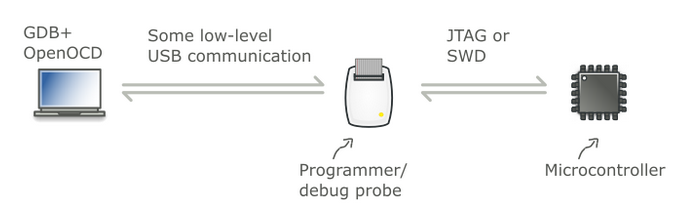
\includegraphics[width=0.9\textwidth]{pc_to_mcu.png}
    \caption{Способ подключения к микроконтроллеру от компьютера.}
\end{figure}


\subsubsection{Инструменты создания образа файловой системы}
В данной работе для создания и организации файловой системы во флеш-памяти микроконтроллера использовался проект SPIFFS.  Для создания образа файловой системы использовался проект mkspiffs, который реализует функции SPIFFS используя стандартную библиотеку С. Проект mkspiffs таким образом позволяет создать образ файловой системы из файлов в директории. После чего данных образ загружается во флеш-память модуля по определенному адресу.


\subsubsection{Цикл разработки}
Одна итерация разработки выглядела следующим образом. Сначала вносились изменения в файлы проекта, неважно пользовательской прошивки или официального SDK. После этого запускалась компиляция программы. При условии успешной компиляции, происходил запуск скрипта-настройщика для OpenOCD. После старта OpenOCD процессса, запускался скрипт-настройщик для GDB. Данный скрипт командовал GDB подключиться к процессу OpenOCD и инициировать загрузку .bin файла во флеш память. Данная процедура была необходима, поскольку программа OpenOCD предоставляет канал между GDB и микроконторллером, а GDB известно какие команды применимы для ядра ARM Cortex-M3 чтобы загрузить бинарный файл во флеш-память. 

\subsubsection{Использование языка Rust}
В данной работе исследовалась возможность программирования микроконторллера на языке Rust, в качестве более безопасной альтернативы языку C.

Безопасность и надежность всегда являются первостепенными задачами. Если прошивка была бы написана на языке программирования Rust, это ограничило бы количество ошибок связанных с переполнением буфера, стека и ряда других типичных для приложений написанных на языке C. Использование Rust также должно было бы упростить тестирование, поскольку юнит-тесты являются частью языка, что будет способствовать поддержанию качество кода. Использование Wi-Fi модуля на основе ARM означает, что Rust может использоваться в качестве языка программирования.

К сожалению задача компиляции языка Rust для данной платформы, а также его интеграция с SDK и уже созданными модулями написаными на С, оказались не тривиальны. Во-первых, для компиляции требовалось подключить LLVM ARM Toolchain, во-вторых многие функции на языке С переопределяются макросами препроцессора, в частности это касается стандартной библиотеки и проекта FreeRTOS, для которых приходится создавать оберточные функции. Это требует больших трудозатрат. После долгих экспериментов пришлось отказаться от использования языка Rust в данной работе.



\subsection{Реализация одно-страничного веб-приложения}
Необходимо учитывать тот факт, что флеш-память ограничена 2 МБ.

\subsubsection{Набор инструментов разработки}
Для разработки использовался текстовый редактор VIM. Система контроля версий Git. Используемые технологии Javascript, CSS, HTML.

\subsubsection{Используемые библиотеки}
Вначале разработки использовалась библиотека Twitter Bootstrap, однако впоследствии от нее пришлось отказаться из-за ее большого размера и вести разработку на более низком уровне.
Также на первых этапах разработки для показа диалогового окна использовалась библиотека tingle, которая впоследствии была заменена на внутренную библиотеку.

\subsubsection{Система сборки}
Задажей системы сборки является из проверить входные файлы на корректность (lint), скомпановать исходники, ужать картинки, оптимизировать шрифты и заархивировав поместить в каталог /dist готовые файлы для веб-приложения.

Для сборки используется система Gulp. В процессе сборки задействовано огромное количество nodejs плагинов. 
Система сборки является одной из самых сложных и многоуровневых частей веб-приложения. 

На первом этапе HTML проходит строгую проверку на корректность и на качество кода. Проверяются от ошибки в опечатках названий элементов до стиля написания id аттрибутов (всегда низкие буквы через нижнее подчеркивание). Для проверки используется пакет htmlhint. 
Ниже представленна конфигурация для запуска htmlmin.

\begin{small}
\begin{verbatim}
    var htmlhintconfig = {
        "tagname-lowercase": true,
        "attr-lowercase": true,
        "attr-value-double-quotes": true,
        "attr-value-not-empty": false,
        "attr-no-duplication": true,
        "doctype-first": true,
        "tag-pair": true,
        "tag-self-close": false,
        "spec-char-escape": true,
        "id-unique": true,
        "src-not-empty": true,
        "title-require": true,
        "alt-require": true,
        "doctype-html5": true,
        "id-class-value": "underscore",
        "style-disabled": false,
        "inline-style-disabled": false,
        "inline-script-disabled": false,
        "space-tab-mixed-disabled": "space",
        "id-class-ad-disabled": false,
        "href-abs-or-rel": false,
        "attr-unsafe-chars": true,
        "head-script-disabled": true
    };
\end{verbatim}
\end{small}


После этого в элемент <head> вставляются два аттрибута с текущей датой-временем и хеш значением последнего коммита в системе Git. Далее в файле заменяются ссылки на файлы .css и .js так как в процессе сборки некоторые файлы будут объеденены в один модуль. Следующим шагом является копирование преобразованного HTML в каталог /debug. Последний шаг это оптимизация HTML удаляющая комментарии с пробелы где это возможно и копирование файла в каталог /dist. 

Следующий шаг - создание единой картинки-спрайта из нескольких картинок которые необходимы в веб-интерфейсе. На данном этапе все картинки PNG объединяются в одну. Оптимизации еще не применяются.
На выходе в каталоге появляется единая картинка spritesheet-bundle.png и .css файл описывающий положение и размер каждой из картинок на единой картинке-спрайте.

После создания единой картинки-спрайта идет верификация и сборка файлов CSS.  

Для верификации CSS используется программа PostCSS и набор плагинов к ней. В частности используется плагин Browserlist для задания списка поддерживаемых браузеров. Список браузеров необходим для плагина Autoprefix который автоматически добавляет префиксы к определенным дескрипторам CSS, если дескрипторы без префикса не поддерживаются в заявленных браузерах.

Далее модули разделяются на те которые были импортированы в проект, например reset.css который разрабатываетяс сообществом, и те модули которые были разработаны для проекта. Инпортированные модули не проходят дополнительные проверки, кроме Autoprefix. После этого они минифицируются с помощю программы clean-css и цопируются в каталоги /debug и /dist.
Модули css которые были созданны в рамках данного проекта подвергаются дополнительной обработке. Во-первых, в модулях используются специальные директивы, которые не входят в стандарт CSS, данные директивы обрабатываются PostCSS плагинам simplevars, который позволяет объявлять переменные в css модулях, и nestedcss, который позволяет писать более простые для понимания вложенные css стили. Данные плагины позволяют расширить синтаксис CSS для упрощения разработки и поддержки кода. После работы данных двух плагинов, запускается еще один PostCSS плагин - stylelint, который проверяет css на корректность и качество кода. Ниже приведена конфигурация плагина stylelint.

\begin{small}
\begin{verbatim}
    var lintconfig = {
        ignoreFiles: [
            // ignore sprites css file generated by spritesmith tool
            'spritesheet.css',
        ],
        rules: {
            // the stylelint-config-recommended, it turns on all the possible errors rules within stylelint
            "at-rule-no-unknown": true,
            "block-no-empty": true,
            "color-no-invalid-hex": true,
            "comment-no-empty": true,
            "declaration-block-no-duplicate-properties": [
                true,
                {
                    ignore: ["consecutive-duplicates-with-different-values"]
                }
            ],
            "declaration-block-no-shorthand-property-overrides": true,
            "font-family-no-duplicate-names": true,
            "font-family-no-missing-generic-family-keyword": true,
            "function-calc-no-unspaced-operator": true,
            "function-linear-gradient-no-nonstandard-direction": true,
            "keyframe-declaration-no-important": true,
            "media-feature-name-no-unknown": true,
            "no-descending-specificity": true,
            "no-duplicate-at-import-rules": true,
            "no-duplicate-selectors": true,
            "no-empty-source": true,
            "no-extra-semicolons": true,
            "no-invalid-double-slash-comments": true,
            "property-no-unknown": true,
            "selector-pseudo-class-no-unknown": true,
            "selector-pseudo-element-no-unknown": true,
            "selector-type-no-unknown": true,
            "string-no-newline": true,
            "unit-no-unknown": true,
            // the stylelist-config-standart, turns on additional rules to enforce common stylistic conventions
            "at-rule-empty-line-before": [ "always", {
                except: [
                    "blockless-after-same-name-blockless",
                    "first-nested",
                ],
                ignore: ["after-comment"],
            } ],
            "at-rule-name-case": "lower",
            "at-rule-name-space-after": "always-single-line",
            "at-rule-semicolon-newline-after": "always",
            "block-closing-brace-empty-line-before": "never",
            "block-closing-brace-newline-after": "always",
            "block-closing-brace-newline-before": "always-multi-line",
            "block-closing-brace-space-before": "always-single-line",
            "block-opening-brace-newline-after": "always-multi-line",
            "block-opening-brace-space-after": "always-single-line",
            "block-opening-brace-space-before": "always",
            "color-hex-case": "lower",
            "color-hex-length": "short",
            "comment-empty-line-before": [ "always", {
                except: ["first-nested"],
                ignore: ["stylelint-commands"],
            } ],
            "comment-whitespace-inside": "always",
            "custom-property-empty-line-before": [ "always", {
                except: [
                    "after-custom-property",
                    "first-nested",
                ],
                ignore: [
                    "after-comment",
                    "inside-single-line-block",
                ],
            } ],
            "declaration-bang-space-after": "never",
            "declaration-bang-space-before": "always",
            "declaration-block-semicolon-newline-after": "always-multi-line",
            "declaration-block-semicolon-space-after": "always-single-line",
            "declaration-block-semicolon-space-before": "never",
            "declaration-block-single-line-max-declarations": 1,
            "declaration-block-trailing-semicolon": "always",
            "declaration-colon-newline-after": "always-multi-line",
            "declaration-colon-space-after": "always-single-line",
            "declaration-colon-space-before": "never",
            "declaration-empty-line-before": [ "always", {
                except: [
                    "after-declaration",
                    "first-nested",
                ],
                ignore: [
                    "after-comment",
                    "inside-single-line-block",
                ],
            } ],
            "function-comma-newline-after": "always-multi-line",
            "function-comma-space-after": "always-single-line",
            "function-comma-space-before": "never",
            "function-max-empty-lines": 0,
            "function-name-case": "lower",
            "function-parentheses-newline-inside": "always-multi-line",
            "function-parentheses-space-inside": "never-single-line",
            "function-whitespace-after": "always",
            "indentation": 4,
            "length-zero-no-unit": true,
            "max-empty-lines": 1,
            "media-feature-colon-space-after": "always",
            "media-feature-colon-space-before": "never",
            "media-feature-name-case": "lower",
            "media-feature-parentheses-space-inside": "never",
            "media-feature-range-operator-space-after": "always",
            "media-feature-range-operator-space-before": "always",
            "media-query-list-comma-newline-after": "always-multi-line",
            "media-query-list-comma-space-after": "always-single-line",
            "media-query-list-comma-space-before": "never",
            "no-eol-whitespace": true,
            "no-missing-end-of-source-newline": true,
            "number-leading-zero": "always",
            "number-no-trailing-zeros": true,
            "property-case": "lower",
            "rule-empty-line-before": [ "always-multi-line", {
                except: ["first-nested"],
                ignore: ["after-comment"],
            } ],
            "selector-attribute-brackets-space-inside": "never",
            "selector-attribute-operator-space-after": "never",
            "selector-attribute-operator-space-before": "never",
            "selector-combinator-space-after": "always",
            "selector-combinator-space-before": "always",
            "selector-descendant-combinator-no-non-space": true,
            "selector-list-comma-newline-after": "always",
            "selector-list-comma-space-before": "never",
            "selector-max-empty-lines": 0,
            "selector-pseudo-class-case": "lower",
            "selector-pseudo-class-parentheses-space-inside": "never",
            "selector-pseudo-element-case": "lower",
            "selector-pseudo-element-colon-notation": "double",
            "selector-type-case": "lower",
            "unit-case": "lower",
            "value-list-comma-newline-after": "always-multi-line",
            "value-list-comma-space-after": "always-single-line",
            "value-list-comma-space-before": "never",
            "value-list-max-empty-lines": 0,
            // our rules, place below
            "property-no-vendor-prefix": true,
            "selector-no-vendor-prefix": true,
            "at-rule-no-vendor-prefix": true,
            "value-no-vendor-prefix": true,
            "declaration-no-important": true,
        }
    };
\end{verbatim}
\end{small}

 Далее css модули проверяются на наличие директив которые появились в последних версиях стандарта CSS и которые не обрабатываются на более старых версиях браузеров. Данная проверка осуществляетяс с помощю PostCSS плагина doiuse, который опирается на базу данных проектов Caniuse и Browserlist. 
 
 
Модули которые были разработаны в рамках данного проекта также обрабатываются плагином Autoprefix. Наконец css копируется в каталог /debug и его минифицированная версия копируются в каталог /dist. Ниже приведены насторйки для данной проверки. Браузер OperaMini исключен из списка, поскольку информация о нем, которая имеется в проектах Caniuse и Browserlist не соответствует действительности. Это вызывает большое количество ложных предупреждений.  

\begin{small}
\begin{verbatim}
var ourbrowsers = ['> 0.05% in RU', 'not ie < 10', 'not OperaMini all'];
\end{verbatim}
\end{small}


После сборки CSS модулей, производится сборка Javascript модулей. Так же как и в случае сборки CSS модулей, несколько Javascript файлов могут объединятся в один модуль. После этого для модулей которые взяты из сообщества, как наприер fullcalendar.js, без дополнительных проверок создаются две копии, вторая из которых минимизируется и файлы копируются в каталоги /debug и /dist для неминифицированной и минифицированной версии соответственно. Модули были написаны в рамках данной работы, подвергаются дополнительной проверке с помосщю программы eslint. Ниже приведена конфигурация для eslint.  

\begin{small}
\begin{verbatim}
    var eslintconf = {
        rules: {
            "accessor-pairs": "off",
            "array-bracket-newline": "off",
            "array-bracket-spacing": "off",
            "array-callback-return": "off",
            "array-element-newline": "off",
            "arrow-body-style": "off",
            "arrow-parens": "off",
            "arrow-spacing": "off",
            "block-scoped-var": "off",
            "block-spacing": "off",
            "brace-style": "off",
            "callback-return": "off",
            "camelcase": "off",
            "capitalized-comments": "off",
            "class-methods-use-this": "off",
            "comma-dangle": "off",
            "comma-spacing": "off",
            "comma-style": "off",
            complexity: "off",
            "computed-property-spacing": "off",
            "consistent-return": "off",
            "consistent-this": "off",
            "constructor-super": "warn",
            curly: "off",
            "default-case": "off",
            "dot-location": "off",
            "dot-notation": "off",
            "eol-last": "off",
            eqeqeq: "off",
            "func-call-spacing": "off",
            "func-name-matching": "off",
            "func-names": "off",
            "func-style": "off",
            "function-paren-newline": "off",
            "generator-star-spacing": "off",
            "getter-return": "off",
            "global-require": "off",
            "guard-for-in": "off",
            "handle-callback-err": "off",
            "id-blacklist": "off",
            "id-length": "off",
            "id-match": "off",
            "implicit-arrow-linebreak": "off",
            indent: "off",
            "indent-legacy": "off",
            "init-declarations": "off",
            "jsx-quotes": "off",
            "key-spacing": "off",
            "keyword-spacing": "off",
            "line-comment-position": "off",
            "linebreak-style": "off",
            "lines-around-comment": "off",
            "lines-around-directive": "off",
            "lines-between-class-members": "off",
            "max-depth": "off",
            "max-len": "off",
            "max-lines": "off",
            "max-nested-callbacks": "off",
            "max-params": "off",
            "max-statements": "off",
            "max-statements-per-line": "off",
            "multiline-comment-style": "off",
            "multiline-ternary": "off",
            "new-cap": "off",
            "new-parens": "off",
            "newline-after-var": "off",
            "newline-before-return": "off",
            "newline-per-chained-call": "off",
            "no-alert": "off",
            "no-array-constructor": "off",
            "no-await-in-loop": "off",
            "no-bitwise": "off",
            "no-buffer-constructor": "off",
            "no-caller": "off",
            "no-case-declarations": "warn",
            "no-catch-shadow": "off",
            "no-class-assign": "warn",
            "no-compare-neg-zero": "warn",
            "no-cond-assign": "warn",
            "no-confusing-arrow": "off",
            "no-console": "warn",
            "no-const-assign": "warn",
            "no-constant-condition": "warn",
            "no-continue": "off",
            "no-control-regex": "warn",
            "no-debugger": "warn",
            "no-delete-var": "warn",
            "no-div-regex": "off",
            "no-dupe-args": "warn",
            "no-dupe-class-members": "warn",
            "no-dupe-keys": "warn",
            "no-duplicate-case": "warn",
            "no-duplicate-imports": "off",
            "no-else-return": "off",
            "no-empty": "warn",
            "no-empty-character-class": "warn",
            "no-empty-function": "off",
            "no-empty-pattern": "warn",
            "no-eq-null": "off",
            "no-eval": "off",
            "no-ex-assign": "warn",
            "no-extend-native": "off",
            "no-extra-bind": "off",
            "no-extra-boolean-cast": "warn",
            "no-extra-label": "off",
            "no-extra-parens": "off",
            "no-extra-semi": "warn",
            "no-fallthrough": "warn",
            "no-floating-decimal": "off",
            "no-func-assign": "warn",
            "no-global-assign": "warn",
            "no-implicit-coercion": "off",
            "no-implicit-globals": "off",
            "no-implied-eval": "off",
            "no-inline-comments": "off",
            "no-inner-declarations": "warn",
            "no-invalid-regexp": "warn",
            "no-invalid-this": "off",
            "no-irregular-whitespace": "warn",
            "no-iterator": "off",
            "no-label-var": "off",
            "no-labels": "off",
            "no-lone-blocks": "off",
            "no-lonely-if": "off",
            "no-loop-func": "off",
            "no-magic-numbers": "off",
            "no-mixed-operators": "off",
            "no-mixed-requires": "off",
            "no-mixed-spaces-and-tabs": "warn",
            "no-multi-assign": "off",
            "no-multi-spaces": "off",
            "no-multi-str": "off",
            "no-multiple-empty-lines": "off",
            "no-native-reassign": "off",
            "no-negated-condition": "off",
            "no-negated-in-lhs": "off",
            "no-nested-ternary": "off",
            "no-new": "off",
            "no-new-func": "off",
            "no-new-object": "off",
            "no-new-require": "off",
            "no-new-symbol": "warn",
            "no-new-wrappers": "off",
            "no-obj-calls": "warn",
            "no-octal": "warn",
            "no-octal-escape": "off",
            "no-param-reassign": "off",
            "no-path-concat": "off",
            "no-plusplus": "off",
            "no-process-env": "off",
            "no-process-exit": "off",
            "no-proto": "off",
            "no-prototype-builtins": "off",
            "no-redeclare": "warn",
            "no-regex-spaces": "warn",
            "no-restricted-globals": "off",
            "no-restricted-imports": "off",
            "no-restricted-modules": "off",
            "no-restricted-properties": "off",
            "no-restricted-syntax": "off",
            "no-return-assign": "off",
            "no-return-await": "off",
            "no-script-url": "off",
            "no-self-assign": "warn",
            "no-self-compare": "off",
            "no-sequences": "off",
            "no-shadow": "off",
            "no-shadow-restricted-names": "off",
            "no-spaced-func": "off",
            "no-sparse-arrays": "warn",
            "no-sync": "off",
            "no-tabs": "off",
            "no-template-curly-in-string": "off",
            "no-ternary": "off",
            "no-this-before-super": "warn",
            "no-throw-literal": "off",
            "no-trailing-spaces": "off",
            "no-undef": "warn",
            "no-undef-init": "off",
            "no-undefined": "off",
            "no-underscore-dangle": "off",
            "no-unexpected-multiline": "warn",
            "no-unmodified-loop-condition": "off",
            "no-unneeded-ternary": "off",
            "no-unreachable": "warn",
            "no-unsafe-finally": "warn",
            "no-unsafe-negation": "warn",
            "no-unused-expressions": "off",
            "no-unused-labels": "warn",
            "no-unused-vars": "warn",
            "no-use-before-define": "off",
            "no-useless-call": "off",
            "no-useless-computed-key": "off",
            "no-useless-concat": "off",
            "no-useless-constructor": "off",
            "no-useless-escape": "warn",
            "no-useless-rename": "off",
            "no-useless-return": "off",
            "no-var": "off",
            "no-void": "off",
            "no-warning-comments": "off",
            "no-whitespace-before-property": "off",
            "no-with": "off",
            "nonblock-statement-body-position": "off",
            "object-curly-newline": "off",
            "object-curly-spacing": "off",
            "object-property-newline": "off",
            "object-shorthand": "off",
            "one-var": "off",
            "one-var-declaration-per-line": "off",
            "operator-assignment": "off",
            "operator-linebreak": "off",
            "padded-blocks": "off",
            "padding-line-between-statements": "off",
            "prefer-arrow-callback": "off",
            "prefer-const": "off",
            "prefer-destructuring": "off",
            "prefer-numeric-literals": "off",
            "prefer-promise-reject-errors": "off",
            "prefer-reflect": "off",
            "prefer-rest-params": "off",
            "prefer-spread": "off",
            "prefer-template": "off",
            "quote-props": "off",
            quotes: ["warn", "single"],
            radix: "off",
            "require-await": "off",
            "require-jsdoc": "off",
            "require-yield": "warn",
            "rest-spread-spacing": "off",
            semi: "warn",
            "semi-spacing": "off",
            "semi-style": "off",
            "sort-imports": "off",
            "sort-keys": "off",
            "sort-vars": "off",
            "space-before-blocks": "off",
            "space-before-function-paren": "off",
            "space-in-parens": "off",
            "space-infix-ops": "off",
            "space-unary-ops": "off",
            "spaced-comment": "off",
            strict: ["warn", "global"],
            "switch-colon-spacing": "off",
            "symbol-description": "off",
            "template-curly-spacing": "off",
            "template-tag-spacing": "off",
            "unicode-bom": "off",
            "use-isnan": "warn",
            "valid-jsdoc": "off",
            "valid-typeof": "warn",
            "vars-on-top": "off",
            "wrap-iife": "off",
            "wrap-regex": "off",
            "yield-star-spacing": "off",
            yoda: "off",
        },
        "globals": [
            "flatpickr",
            "vline",
            "DataView",
        ],
        "envs": [
            "browser"
        ],
    };
\end{verbatim}
\end{small}


Следующим шагом в каталоги /debug и /dist копируются дополнительные файлы необходимые для правильной работы веб-приложения. В частности это шрифты и изображения.

Следуюшим шагом записакется одна из самых значимых оптимизаций, а именно оптимизация шрифтов. Файлы шрифтов предствленны в 3-х форматах TTF (True Type Font), EOT (Embedded Open Type), WOFF (Web Optimised Font Format) для обеспечения кросс-браузрного функционирования. Для оптимизации шрифтов используется программа fontmin. Она удаляет из файлов со шрифтами неиспользуемые глифы (glyph).

После этого файлы в каталоге /debug можно использовать для отладки и тестирования веб-прилочения. Файлы в каталоге /dist проходят через дополнительные этапы. В частности все ссылки на файлы типа css, js, html, svg, woff, ttf, png модифицируются добавлением хеш значения от последнего Git коммита. Это позволяет управлять кешированием в браузере и существенно влияет на взаимодействие пользователя с программой, поскольку повторное подключение проишодит мгновенно т.к. использует кеш браузера и не требует полной загрузки всех файлов приложения с РВ-90.    

Далее проишодит оптимизация единого изображения spritesheet-bundle.png. Для этого используется программа imagemin. Альтернативными программами являются pngquant и imageoptim. Хотя pngquant давал результат чуть лучше чем imagemin, в системе сборки используется именно imagemin, т.к. он лучше интегрирован с экосистемой nodejs и npm, это важный параметр поскольку такая интеграция делает систему сборки переносимой между разными операционными системами. 

Последним этапом сборки является архивирование всех модулей, и шрифтов SVG. Для архивации используется программа zopfli. Формат архивации совместим с программой gzip, однако архиватор zopfli показал более высокую степень сжатия файлов.

\subsubsection{Цикл разработки}
Цикл разработки выглядит следующим образом. Первая сборка проекта производится вручную. Далее в папке /debug также вручную запускается предельно простой HTTP сервер реализованный на языке Python и поставляемый вместе с проектом. После этого система сборки Gulp переходит в режим watch. В данном режиме Gulp отслеживает изменения в ишодных файла и автоматически пересобирает проекта. Проверка и отладка веб приложения производятся в браузере, который подключается к HTTP серверу запущенному в папке /debug. 


\subsection{Реализация мобильного приложения}

\subsubsection{Инструменты разработки}
Вся разработка велась в AndroidStudio IDE. Официальном средстве разработки для системы Android от компании Google.

\subsubsection{Используемые библиотеки}
Для реализации Android приложения были использованны несколько библиотек находящихся в открытом доступе. В частности для реализации Controls календаря и цикла реле были использованны существенно модифицированные вверсии CalendarLibrary и 24hAnalogWidget. Для взаимодействия с сетью и премом/передачи JSON была использована библиотека Retrofit. Для создания Layout в активити отражающем все календари и все циклы календаря, использовался открытый код проекта - Flexbox. Также при выборе названия для цикла у пользователя есть возможность выбрать и цвет. Для выбора цвета использовался открытый проект Colorpicker.

\subsubsection{Цикл разработки}
Использовался стандартный цикл разработки подходясщих для большинства мобильных приложений.

\newpage
\section{Заключение}
\subsection{Ориeнтировочная экономическая эффективность}
Ориeнтировочная экономическая эффективность не рассчитывается.

\subsection{Экономические преимущества разработки}
Ориeнтировочны экономические преимущества разработки не рассчитывается.

\newpage
\section{Источники, используемые при разработке}
\subsection{Список используемой литературы}
\begin{my_enumerate}

\item
Bellard Fabrice. QEMU, a Fast and Portable Dynamic Translator //
Proceedings of the Annual Conference on USENIX Annual Technical Conference. 2005.

\item
ГОСТ 19.103-77 Обозначения программ и программных документов. // Единая система программной документации. -М.: ИПК Издательство стандартов, 2001. \\

\item
ГОСТ 19.104-78 Основные надписи // Единая система программной документации. -М.: ИПК Издательство стандартов, 2001. \\

\item
ГОСТ 19.105-78 Общие требования к программным документам. // Единая система
программной документации. – М.: ИПК Издательство стандартов, 2001. \\


\end{my_enumerate}



% Index
\newpage

\eskdListOfChanges

% \phantomsection
% \addcontentsline{toc}{section}{Алфавитный указатель}
% \printindex

\end{document}
